\documentclass[a4paper]{report}
\usepackage[utf8x]{inputenc}
\usepackage[portuges]{babel}
\usepackage{graphicx}
\usepackage{lipsum}
\usepackage{color}
\usepackage{listings}
\usepackage{float}
\setlength{\parskip}{1em}
\lstset{language=Haskell,basicstyle=\footnotesize,numbers=left,numberstyle=\footnotesize,stepnumber=1,numbersep=5pt,backgroundcolor=\color{white},showspaces=false,showstringspaces=false,showtabs=false,frame=single,tabsize=2,captionpos=b,breaklines=true,breakatwhitespace=false,escapeinside={\%*}{*)}}

\begin{document}


\title{Relatório Trabalho Prático LI1}
\author{Grupo 05\\
\\
Hugo Cardoso e João Cunha}
\date{\today}

\maketitle

\tableofcontents

\listoffigures

\chapter{Introdução}

\section{Contextualização}

A unidade curricular de Laboratórios de Informática I consiste no desenvolvimento de um projeto ao longo de todo o semestre, que se resume à criação de um jogo. O projeto deste ano (2017/18) traduz-se no desenvolvimento de um jogo de corridas de carros, sendo necessário para a realização do mesmo a aplicação de conhecimentos de várias áreas, nomeadamente a programação e a física.

O projeto encontra-se dividido em duas fases e seis tarefas. Em cada fase, é expectável a realização de três tarefas, sendo distribuído um enunciado por fase com instruções e orientações acerca das mesmas. As tarefas estão organizadas de forma lógica segundo a sua relevância para o trabalho, dificuldade e complexidade. É ainda esperado o desenvolvimento de um relatório na segunda fase, a explanar todo o raciocínio por detrás da resolução do projeto.

\section{Motivação}

Com este projeto, pretende-se que os alunos adquiram várias bases para todo o curso e, em especial, para futuras cadeiras da área da programação. Em primeiro lugar, é esperado um grande desenvolvimento na capacidade de uso da linguagem de programação \textit{Haskell}, lecionada em Programação Funcional, em paralelo com esta unidade curricular. Com isto, entende-se também a aprendizagem de documentação (e leitura de documentação de) código e do uso do sistema de partilha de código \textit{SVN}. Todavia, para além disto, tem-se também por objetivo que os estudantes desenvolvam a habilidade de trabalhar em equipa, dividindo tarefas e responsabilidades, de cumprir horários e respeitar datas de entrega e de redigir relatórios (aprendendo também a usar softwares especializados para esse fim - \textit{LaTeX}), um elemento fundamental a qualquer trabalho prático.

\section{Objetivos}

O objetivo do projeto da unidade curricular de Laboratórios de Informática I este ano é implementar o clássico jogo de corridas Micro Machines. A principal meta do jogo é completar um percurso pré-definido no menor tempo possível. Este percurso pode ter alturas diferentes e é rodeado por lava, sendo o jogador penalizado sempre que sofre uma queda dentro do percurso ou quando cai na lava.

As tarefas que constituem o projeto seguem a seguinte lógica: construir mapas que serão posteriormente validados, implementar o carro e as suas interações com o mapa, efetuar uma maneira de os jogadores controlarem os carros, programar graficamente o jogo e, por fim, construir um carro que corra sozinho.

\chapter{Análise de Requisitos}

\section{Fase 1}

\subsection{Tarefa 1 - Construir Mapas}

A Tarefa 1 consiste na construção de mapas, partindo de caminhos previamente definidos. O caminho consiste no conjunto de passos que o carro tem de dar para completar o percurso.

\begin{verbatim}
    data Passo = Avanca | Sobe | Desce | CurvaDir | CurvaEsq
\end{verbatim}

O mapa consiste numa matriz de peças, que podem variar em altura (as peças lava têm altura fixa de 0) e orientação (há peças que não têm orientação). 

\begin{verbatim}
    type Altura = Int
    data Peca = Norte | Sul | Este | Oeste
\end{verbatim}

A construção do tabuleiro deve começar a partir da posição inicial dada pela função \textit{partida} e, nesta tarefa em específico, na direção Este e com a altura 0. O tabuleiro deve apresentar a dimensao dada pela função \textit{dimensao} e todas as posições não percorridas pelo caminho devem ser preenchidas por peças lava. Caso o caminho passe pela mesma posição mais do que uma vez, deve ser considerado o resultado do passo mais recente. \par
Assim, o objetivo desta tarefa resume-se a definir uma função \textit{constroi} que, recebendo um caminho constrói o mapa correspondente.

\begin{verbatim}
    data Mapa = Mapa (Posicao,Orientacao) Tabuleiro
\end{verbatim}

\subsection{Tarefa 2 - Validar Mapas}
\label{analisetarefa2}

Esta tarefa tem o propósito de testar se um dado mapa é ou não válido. Para isto, o mapa tem de obedecer a um conjunto de regras que asseguram que existe um percurso de peças que permite ao carro dar voltas à pista. As regras são as seguintes:

\begin{enumerate}
    \item Existe um único percurso e todas as peças fora desse percurso são do tipo lava;
    \item O percurso deve corresponder a uma trajetória, tal que começando na peça de partida com a orientação inicial, volta-se a chegar à mesma com a orientação inicial;
    \item A orientação inicial tem que ser compatível com a peça de partida. Isto verifica-se apenas se for possível entrar na peça seguindo essa orientação (esta questão só é relevante para as peças do tipo curva e rampa;
    \item As peças do percurso só podem estar ligadas a peças do percurso com alturas compatíveis;
    \item Todas as peças do tipo lava estão à altura 0;
    \item O mapa é sempre retangular e rodeado por lava, isto é, a primeira e última linha, bem como a primeira e última coluna, são necessariamente constituídas por peças do tipo lava.
\end{enumerate}

Resumindo, o objetivo desta tarefa é definir a função \textit{valida} que, dado um mapa, verifica se o mesmo é válido ou não. Além disso, considera-se ainda que o percurso pode começar a uma altura, numa direção e numa posição diferentes das consideradas na Tarefa 1.

\subsection{Tarefa 3 - Movimentar o Carro}
\label{analisetarefa3}

O propósito da Tarefa 3 é começar a implementar a mecânica do jogo, isto é, as movimentações do carro no mapa de jogo e as respetivas colisões com obstáculos. Como tal, modela-se um \textit{Carro} como contendo um posicao (representada por um ponto, uma posição com decimais), uma direção (um ângulo em graus) e um vetor de velocidade:

\begin{verbatim}
    data Carro = {posicao :: Ponto
                 ,direcao :: Angulo
                 ,velocidade :: Velocidade}
\end{verbatim}
 Pretende-se então calcular o novo estado de um carro após um determinado período de tempo, dado o seu estado atual. Como tal, deve-se ter as mente as interações com o mapa que podem ocorrer nesse período de tempo:
 
 \begin{itemize}
     \item Se o carro transita para a lava é "\textit{destruído}";
     \item Se o carro transita para uma posição pelo menos uma unidade mais baixa que a atual, então "\textit{cai}" ou é "\textit{destruído}", dependendo se passa para outra peça do percurso ou para uma peça do tipo lava;
     \item Se o carro transita para uma posição pelo menos uma unidade mais alta que a atual, então \textit{colide} contra a peça, devendo ser calculado o impacto da colisão, ou seja, qual o respetivo "\textit{ricochete}";
     \item Se o carro transita entre duas posições com diferença de alturas menor que uma unidade, então movimenta-se normalmente.
 \end{itemize}

Desta forma, durante o período de tempo dado, a mesma interação pode repetir-se e podem ocorrer diferentes tipos de interação. Contudo, assume-se sempre que o carro está numa posição válida, ou seja, dentro do percurso. Deve também ter-se em conta o seguinte:

\begin{itemize}
    \item A direção do carro não é alterada nesta tarefa;
    \item O carro desloca-se a velocidade constante, não "acelerando" nem "curvando", inclusive durante colisões. Mais concretamente, o "valor absoluto" da velocidade não é alterado, mas sim a sua direção de acordo com o ângulo de colisão.
\end{itemize}

Logo, o objetivo desta tarefa é definir a função \textit{movimenta} que, dado um tabuleiro, um tempo e um carro, devolve o novo estado do carro sob a forma de um \textit{Maybe Carro}. Desta forma, a função deve retornar um \textit{Nothing} quando o carro é "\textit{destruído}" ou um \textit{Just e}, caso contrário, sendo \textit{e} o novo estado do carro.

\section{Fase 2}

\subsection{Tarefa 4 - Atualizar Estado}
\label{analisetarefa4}

O objetivo desta tarefa é atualizar o estado do jogo dadas as ações efetuadas pelo jogador num período de tempo. Para esse fim é necessário representar:
 
\begin{itemize}
    \item \textbf{Jogo} - o estado interno do jogo (que deverá ser atualizado em cada instante);
    \item \textbf{Ação} - algo que vai indicar, por exemplo, se o carro está a acelerar, travar ou curvar.
\end{itemize}

\subsubsection{Estado do Jogo}

O estado do jogo é definido em cada momento por um mapa e as suas propriedades, bem como listas com os estados dos carros, as quantidades de "\textit{nitro}" disponíveis e os \textit{históricos} de todas as posições visitadas. Estas lista devem ter a mesma dimensão, correspondente ao número de jogadores.

\begin{verbatim}
    data Jogo = Jogo
      { mapa      :: Mapa
      , pista     :: Propriedades
      , carros    :: [Carro]
      , nitros    :: [Tempo]
      , historico :: [[Posicao]]
      }
\end{verbatim}

As propriedades são constantes físicas que afetam o movimento do jogo e que deverão ter sidas em conta para a realização desta tarefa. Variam de percurso para percurso e são definidas da seguinte forma:

\begin{verbatim}
    data Propriedades = Propriedades
      { k_atrito :: Double
      , k_pneus  :: Double
      , k_acel   :: Double
      , k_peso   :: Double
      , k_nitro  :: Double
      , k_roda   :: Double
      }
\end{verbatim}

Uma funcionalidade a ser implementada é a possibilidade de ativar "nitros" sobre qualquer jogador. Cada jogador tem inicialmente disponível uma quantidade limitada de "nitro", que se gasta de cada vez que é ativado pelo jogador.

\subsubsection{Ações do jogador}

As ações do jogador definem se o carro está a \textit{acelerar, travar, curvar para a direita ou esquerda} ou com o "nitro" ativado e têm efeito num dado período de tempo.

\begin{verbatim}
    data Acao = Acao
      { acelerar :: Bool
      , travar   :: Bool
      , esquerda :: Bool
      , direita  :: Bool
      , nitro    :: Maybe Int
      }
\end{verbatim}

Podem ser dadas várias ações ao mesmo tempo, embora os efeitos de algumas delas se anulem (acelerar/travar e esquerda/direita). O nitro representa o possível alvo de um "nitro".

O estado do jogo deve ser atualizado de acordo com o impacto das ações de um determinado jogador no dado período de tempo, recorrendo às propriedades do jogo. De facto, o que se pretende com esta tarefa é:

\begin{itemize}
    \item Atualizar o vetor velocidade do carro;
    \item Atualizar a direção do carro;
    \item Atualizar a quantidade de "nitro" disponível no carro;
    \item Atualizar o histórico de posições percorridas pelo carro.
\end{itemize}

Assim, o objetivo é definir a função \textit{atualiza} que recebe um tempo, um jogo, o identificador de um jogador e a ação realizada pelo mesmo e, com tudo isso, atualiza o estado o jogo. É necessário manter em conta que a posição do carro se deve manter inalterada nesta tarefa, pois a sua atualização já é tratada na tarefa anterior.

\subsection{Tarefa 5 - Implementação do Jogo em Gloss}
\label{analisetarefa5}

A Tarefa 5 consiste na implementação do jogo completo usando a biblioteca Gloss. Apesar de dever ser construída inicialmente sobre as tarefas anteriores, sobretudo as Tarefas 3 e 4, esta tarefa trata-se de uma "tarefa livre", sendo incentivada e valorizada a originalidade e a implementação de novas mecânicas no jogo.

\subsection{Tarefa 6 - Implementar uma Estratégia de Corrida}

Por fim, esta última parte do trabalho prático é dedicada à implementação de um \textit{bot} que jogue Micro Machines automaticamente, isto é, seja capaz de correr contra outros carros e completar o percurso sem receber qualquer \textit{input} dos jogadores. Para definir a estratégia, é necessário assumir que:

\begin{itemize}
    \item O objetivo do jogo é dar uma volta à pista à frente dos adversários, começando e acabando na posição de partida.
    \item O jogo acaba passado 60 segundos, independentemente de algum carro ter conseguido dar a volta, sendo que, nesse caso, o vencedor será o carro mais avançado no percurso.
    \item Os mapas são válidos de acordo com a Tarefa 2, e a física do jogo é a mesma das Tarefas 3 e 4.
    \item Cada jogador começa com 5 segundos de "nitro".
    \item Atalhos são permitidos até 4 peças, sendo o carro destruído se tentar cortar mais caminho do que isso.
    \item Quando o carro é destruído, volta ao centro da última posição visitada com velocidade zero e fica imobilizado durante 1.5 segundos.
    \item O percurso é selecionado a partir de um conjunto fixo de caminhos e propriedades fornecidos pelos docentes.
\end{itemize}

Concluindo, procura-se definir a função \textit{bot} que dada a duração da ação a tomar, o estado do jogo e o identificador do jogador, devolve essa mesma ação.



\chapter{A Nossa Solução}

\section{Fase 1}

\subsection{Tarefa 1}
\label{solucaotarefa1}

A abordagem a esta tarefa começou pela definição de uma função \textit{tabuleiroLava} que constrói um tabuleiro com a dimensão fornecida (obtida através da função \textit{dimensao} predefinida no módulo LI11718) formado apenas por peças do tipo lava, a partir do qual se construiria o tabuleiro final, substituindo as peças nas posições que pertencessem ao percurso.

Como tal, criou-se também a função \textit{atualizarTabuleiroLinha}, que atualiza a peça de uma linha na posição fornecida. Esta serviu como base para uma função que atualiza qualquer posição de um tabuleiro (\textit{atualizarTabuleiro}) que, por sua vez, serviu como intermédio para o desenvolvimento da \textit{atualizarTabuleiroTodo}, que atualiza um qualquer conjunto de peças de um tabuleiro.

\begin{lstlisting}
atualizarTabuleiroTodo :: Tabuleiro -> [Peca] -> [Posicao] -> Tabuleiro
atualizarTabuleiroTodo a [] [] = a
atualizarTabuleiroTodo [] b c = []
atualizarTabuleiroTodo a (h1:t1) (h2:t2) = atualizarTabuleiroTodo (atualizarTabuleiro a h1 h2) t1 t2
\end{lstlisting}

Com isto, falta então perceber que posições pertencerão ao circuito e que peça deverá ter cada uma dessas posições. Definiu-se, portanto, a função \textit{passoParaPeca}. Tal como o nome indica, esta função "transforma" o caminho (lista de passos) numa lista de peças, com auxílio da orientação e posição iniciais. Para tal fim, recorre a várias funções auxiliares que estudam o comportamento das peças e da orientação em curvas (\textit{esqAux} e \textit{dirAux}) e rampas (\textit{sobeAux} e \textit{desceAux}). Por exemplo:

\begin{verbatim}
dirAux :: Orientacao -> Altura -> (Peca,Orientacao)
dirAux Norte a = (Peca (Curva Norte) a, Este)
dirAux Este a  = (Peca (Curva Este) a, Sul)
dirAux Sul a   = (Peca (Curva Sul) a, Oeste)
dirAux Oeste a = (Peca (Curva Oeste) a, Norte)
\end{verbatim}

Pelo mesmo raciocínio, formou-se a função \textit{posicaoPeca} que retorna a lista de posições ocupadas por peças do circuito, a partir dos mesmos parâmetros que a função anterior.

Tudo isto é reunido na última função, \textit{constroi}, que, dado um caminho, retorna o mapa correspondente, que é constituído pela posição e orientação iniciais e pelo tabuleiro.

\begin{verbatim}
constroi :: Caminho -> Mapa 
constroi [] = Mapa (partida [],dirInit) (tabuleiroLava (dimensao []))
constroi c = let
                 x = passoParaPeca c dirInit altInit
                 y = tabuleiroLava (dimensao c)
                 z = partida c : posicaoPeca c (partida c) dirInit
             in 
             Mapa (partida c,dirInit) (atualizarTabuleiroTodo y x z)
\end{verbatim}



\subsection{Tarefa 2}

Como foi referido em \ref{analisetarefa2}, há uma lista de condições que têm de ser verificadas para um mapa ser válido. A primeira que foi abordada foi a última enunciada em \ref{analisetarefa2}, ou seja, a necessidade de o tabuleiro ser rodeado por lava e retangular.

Para este efeito, criou-se a função \textit{rodeadoLava}, que verifica se todas as peças na primeira e última linha são do tipo lava, bem como na primeira e última coluna.

\begin{lstlisting}
rodeadoLava :: Tabuleiro -> Bool
rodeadoLava t =  linhasLava (head t)(last t) && colunasLava t 
    where
        linhasLava [][] = True
        linhasLava (h:t)(h1:t1) = (h == Peca Lava altLava && h1 == Peca Lava altLava) && linhasLava t t1 
        colunasLava [] = True
        colunasLava ((h:t):t1) = (h == Peca Lava altLava && last t == Peca Lava altLava) && colunasLava t1
\end{lstlisting}

Além disso, recorre-se também à função \textit{tabRetangular} que, como o nome sugere, verifica se o tabuleiro é, de facto, retangular.

\begin{verbatim}
tabRetangular :: Tabuleiro -> Bool
tabRetangular [] = True
tabRetangular [h] = True
tabRetangular (h:h1:t) | length h == length h1 = tabRetangular (h1:t)
                       | otherwise = False 
\end{verbatim}

De seguida, fez-se uma função para averiguar se todas as peças do tipo lava estão à altura 0, que percorre o tabuleiro peça a peça e, caso a peça seja do tipo lava, verifica se está à altura 0 ou não, retornando um Booleano.

\begin{verbatim}
valLava :: Tabuleiro -> Bool
valLava [] = True
valLava ([]:t1) = valLava t1
valLava ((Peca Lava a:t):t1) | a == 0 = valLava (t:t1)
                             | otherwise = False
valLava ((_:t):t1) = valLava (t:t1)
\end{verbatim}

Procurou-se verificar os pontos 2,3 e 4 todos de uma só vez, visto que envolviam processos de resolução semelhantes ou interligados e, portanto, mutuamente benéficos.

Basicamente, o raciocínio utilizado passou por determinar a que posições do tabuleiro pertenciam as peças do circuito. Isto é, o raciocínio é em tudo semelhante ao da função \textit{posicaoPeca} descrita em \ref{solucaotarefa1} menos na execução, uma vez que nesta tarefa não se dispunha do caminho, pelo que se teve de partir do tabuleiro em si para chegar à lista das posições, com auxílio da posição e orientação iniciais presentes no mapa a testar.

Com isto em mente, desenvolveu-se a função \textit{verificarTabuleiro}: 

\begin{lstlisting}
verificarTabuleiro :: Posicao -> Orientacao -> Tabuleiro -> Int -> Posicao -> [Posicao] -> Altura -> ([Posicao],Bool) 
verificarTabuleiro (0,0) o l y c a h = ([],False)
verificarTabuleiro p o l y c a h 
   | compPos p c && y /= 0 = (a,True)                       
   | o == Este  =  verificarTabuleiro (primeiro i) (segundo i) l (y+1) c (a++[p]) (terceiro i)                          
   | o == Oeste =  verificarTabuleiro (primeiro j) (segundo j) l (y+1) c (a++[p]) (terceiro j)                          
   | o == Norte =  verificarTabuleiro (primeiro m) (segundo m) l (y+1) c (a++[p]) (terceiro m)                          
   | o == Sul   =  verificarTabuleiro (primeiro n) (segundo n) l (y+1) c (a++[p]) (terceiro n)
  where
    i = oriEste  (buscarPeca p l) p h
    j = oriOeste (buscarPeca p l) p h
    m = oriNorte (buscarPeca p l) p h
    n = oriSul   (buscarPeca p l) p h
\end{lstlisting}

Como podemos observar, esta função começa por recorrer à função \textit{compPos}, que compara duas posições, verificando se são iguais. A função \textit{verificarTabuleiro} vai então comparar a posição inicial do tabuleiro, que vai ser o quinto parâmetro que lhe é fornecida, com a posição da peça em que a função está atualmente (manter em mente que esta função vai percorrer todas as posições cujas peças pertencem ao circuito). Vai parar quando esta comparação for verdadeira, devolvendo o  que representa isso (\textit{True}) e a lista de todas as posições que comparou com a posição de partida até aí, isto é, todas as posições de peças do circuito. Logo, a função \textit{verificarTabuleiro} vai parar apenas depois de percorrer o percurso inteiro. Contudo, como esta função começa na posição de partida, a função \textit{compPos} devolveria logo verdadeiro na sua primeira utilização. Para evitar isto, a \textit{verificarTabuleiro} recebe também um inteiro como parâmetro, ao qual se vai somando uma unidade a cada posição nova do percurso. Adiciona-se também, portanto, a resguarda de que a função só deve parar se o inteiro for diferente de 0, qu é o valor inicial dado:

\begin{verbatim}
verificarTabuleiro p o l y c a h | compPos p c && y /= 0 = (a,True) 
\end{verbatim}

Caso a \textit{compPos} retorne falso, vai-se então averiguar qual a orientação atual. Dependendo desta, chama-se uma de quatro funções auxiliares semelhantes. Por exemplo, se a orientação for Este:

\begin{lstlisting}
oriEste :: Maybe Peca -> Posicao -> Altura -> (Posicao,Orientacao,Altura)
oriEste (Just (Peca (Curva Este) a)) (c,l) h  = if h == a     then ((c,l+1),Sul,h)    else ((0,0),Sul,h)
oriEste (Just (Peca (Curva Sul) a)) (c,l) h   = if h == a     then ((c,l-1),Norte,h)  else ((0,0),Sul,h)
oriEste (Just (Peca (Rampa Este) a)) (c,l) h  = if h == a     then ((c+1,l),Este,h+1) else ((0,0),Sul,h)
oriEste (Just (Peca (Rampa Oeste) a)) (c,l) h = if (h-1) == a then ((c+1,l),Este,h-1) else ((0,0),Sul,h)
oriEste (Just (Peca Recta a)) (c,l) h         = if h == a     then ((c+1,l),Este,h)   else ((0,0),Sul,h)
oriEste _ (c,l) h                             = ((0,0),Sul,h)
\end{lstlisting}

Esta função recebe como parâmetros a peça na posição atual da \textit{verificarTabuleiro}, caso exista, que é obtida pela função \textit{buscarPeca}, a posição e a altura atuais. A função buscarPeca verifica se a posição dada pertence ao tabuleiro, recorrendo à posição \textit{posTabuleiro} e, em caso afirmativo, devolve \textit{Just p}, sendo p a posição em questão, caso contrário devolve \textit{Nothing}. Esta resguarda serve para prevenir a validação de mapas com posições iniciais e tabuleiros incoerentes.

Desta forma, a função \textit{oriEste}, tal como as outras três referidas, devolve a posição da peça seguinte, a orientação que o caminho toma ao entrar na mesma e a altura atualizada. Caso não receba uma peça válida ou a altura atual não seja a mesma que a altura da peça atual, a função devolve um resultado impossível, com a posição (0,0). Como já verificamos anteriormente, essa posição será sempre ocupada por uma peça do tipo Lava. Quando isto ocorre, entra em ação o caso de paragem da \textit{verificarTabuleiro} que, recebendo esta posição, interrompe a função, ficando-se a saber que o mapa é inválido.

\begin{verbatim}
verificarTabuleiro (0,0) o l y c a h = ([],False)
\end{verbatim}

Assim, a função \textit{verificarTabuleiro} vai averiguar se o percurso corresponde a uma trajetória, pois começa na peça de partida e acaba na mesma, verificando se a orientação inicial é igual à orientação com que se volta a chegar à referida peça (condição 2). Acaba, portanto, por verificar também que a orientação inicial é compatível com a peça de partida (ponto 3). Certifica-se, por fim, de que as peças do percurso apenas estão ligadas a peças do percurso com alturas compatíveis, mais especificamente nas funções auxiliares que devolvem os triplos (condição 4). Se a \textit{verificarTabuleiro} devolver \textit{True} como segundo elemento do par, então tudo isto é verdadeiro.

Só resta então assegurar a primeira regra, ou seja, que existe apenas um percurso e todas as peças fora desse percurso são do tipo lava. 

Em primeiro lugar, dá-se a lista de posições das peças do circuito, que é o primeiro elemento do par que a  \textit{verificarTabuleiro} devolve, à função \textit{atualizarTabuleiroTodo}, que é idêntica à função com nome igual da tarefa 1. Esta vai subtituir as peças em todas essas posições por peças do tipo Lava, pelo que deve restar um tabuleiro constituído unicamente por peças do tipo Lava. Caso isto não se verifique, significa que existe pelo menos uma peça não Lava fora do percurso, pelo que o mapa é inválido. É isto que a função \textit{subtracaoTab} faz, fornecendo o tabuleiro resultante da \textit{atualizarTabuleiroTodo} à função \textit{valTudoLava}, que percorre o mesmo peça a peça, verificando se são todas do tipo Lava:

\begin{verbatim}
valTudoLava :: Tabuleiro -> Bool
valTudoLava [] = True
valTudoLava ([]:t1) = valTudoLava t1
valTudoLava ((Peca Lava _:t):t1) = valTudoLava (t:t1)
valTudoLava ((_:t):t1) = False
\end{verbatim}

Tudo o que aqui foi falado culmina na função \textit{valida} que, dada um mapa, verifica se é válido.

\begin{lstlisting}
valida :: Mapa -> Bool
valida (Mapa(p,o) []) = False
valida (Mapa(p,o) t) 
 | partidaDesce p t (hdePartida p t) o = tabRetangular t && posTabuleiro p t && snd(verificarTabuleiro p o t 0 p [] (1+hdePartida p t)) && rodeadoLava t && valLava t && subtracaoTab p o t 0 p [] (1+hdePartida p t)
 | otherwise = tabRetangular t && posTabuleiro p t && snd(verificarTabuleiro p o t 0 p [] (hdePartida p t)) && rodeadoLava t && valLava t && subtracaoTab p o t 0 p [] (hdePartida p t)
\end{lstlisting}

Tal como em \ref{solucaotarefa1}, adiciona-se um caso de paragem à função para quando o tabuleiro é vazio, sendo o mapa não válido nesse caso, obviamente, visto que não há circuito para os carros.

Além disso, é preciso tomar ainda atenção a mais um aspeto. Se o circuito começar numa rampa descendente, a altura da peça inicial vai ser uma unidade abaixo do que é, na realidade, a altura inicial. Desta maneira, a \textit{verificarTabuleiro} vai receber um parâmetro errado, pelo que pode acabar por validar um mapa inválido. Assim, cria-se, por fim, a função \textit{partidaDesce}, que averigua se o referido acontece e, em caso afirmativo, soma uma unidade à altura da peça inicial.

\subsection{Tarefa 3}

O objetivo desta tarefa é implementar as interações do carro com o mapa. Para a eficiente realização do raciocínio desenvolvido, criaram-se dois tipos de dados novos: 

\begin{verbatim}
type Linha = (Ponto,Ponto)

type Parede = ((Int,Int),(Int,Int))
\end{verbatim}

Começa-se por criar uma linha que contém o vetor velocidade do carro. Para este propósito, usa-se a função \textit{vetorCarro}, que devolve a linha constituída pela posição do carro e pela posição resultante da soma do vetor velocidade à posição do carro.

De seguida, calculam-se as "paredes" da peça em que o carro se situa, isto é, os limites da mesma. Qualquer peça tem 4 paredes, superior, inferior, à esquerda e à direita, exceto as peças do tipo curva, que têm apenas 3. Daí se ter adicionado esses "casos de paragem" à função responsável por isto:

\begin{verbatim}
paredes :: Peca -> (Int,Int) -> [Parede]    
paredes (Peca (Curva Este) _)  (x,y) = (...)
paredes (Peca (Curva Sul) _)   (x,y) = (...)
paredes (Peca (Curva Oeste) _) (x,y) = (...)
paredes (Peca (Curva Norte) _) (x,y) = (...)
paredes _ (x,y)                      = (...)
\end{verbatim}

Tendo as paredes da peça, verifica-se quais delas são intersetadas pela linha que contém o vetor velocidade, recorrendo à função \textit{maybeIntersection}, que pode retornar dois tipos de resultados:

\begin{itemize}
    \item O ponto de interseção;
    \item (-100,-100), que é o resultado quando não há interseção entre as linhas.
\end{itemize}

Com isto, fica-se com os pontos em que a linha do vetor velocidade interseta as paredes da peça. Seguidamente, verifica-se quais desses pontos fazem efetivamente parte da peça. Este passo serve tanto para distinguir os pontos de interseção do ponto dado quando as linhas nunca se cruzam como para eliminar os pontos que resultam da interseção, mas não pertencem à peça. Atente-se, por exemplo, no seguinte caso:

\begin{verbatim}
maybeIntersection ((2,2),(3,2)) ((2.5,1.5),(3.5,2))
(3.5,2.0)
\end{verbatim}

Neste exemplo, estamos a intersetar a linha do vetor velocidade com a parede inferior da peça (2,1). O ponto de interseção é (3.5,2.0), ou seja, pertence à peça (3,1), pelo que não faz parte da peça em que o carro se situa. Logo, não deve ser considerado.

Escolhidos os pontos de interseção que fazem parte da peça onde se situa o carro, usa-se a função \textit{pontoIntersecao} que identifica qual dos pontos de interseção é o correto, tendo em conta o sentido do vetor velocidade.

De seguida, a função \textit{qualParede}, com este ponto, o ponto da peça atual do carro e a própria peça, averigua a posição da peça para a qual o carro vai passar a seguir e por onde entrará na mesma (pela direita, por cima, por um canto, etc). Caso a peça em questão seja uma curva, verifica também se o carro está a transitar para a metade da peça constituída por lava, determinando, nesse caso, se o carro é destruído ou se faz ricochete.  Abaixo podemos ver como esta função atua, por exemplo, em Curvas Este:

\begin{verbatim}
qualParede (Peca (Curva Este) h)  (a,b) (x,y)
  | x == a && y == b = ((a-1,b-1),4) -- canto
  | x == (a+1) && y == (b+1) = ((a+1,b-1),4) --canto
  | x == a && y == (b+1) = ((a+1,b+1),4) --canto
  | y == (b+1) = ((a,b+1),7) -- fundo da peça
  | x == a = ((a-1,b),8) -- lado esquerdo
  | h > -1 = ((-1,-1),0) -- destruição
  | otherwise = ((-50,-50),0) -- ricochete
\end{verbatim}

Naturalmente, o próximo passo é determinar o tipo de interação com a próxima peça, caso passe efetivamente para esta (ou seja, exceto nos casos em que se dirige à lava das curvas). Além disso, é necessário perceber se a diferença entre as alturas das peças é maior ou igual a uma unidade, o que significa que o carro "cai" e é destruído. A função \textit{drs} é responsável por isto, devolvendo um inteiro, que pode ser qualquer um dos seguintes:

\begin{enumerate}
    \item Destruição do carro;
    \item Ricochete;
    \item O carro segue em frente.
\end{enumerate}

Caso haja ricochete, calcula-se o novo vetor velocidade, que pode ser identificado através do seguinte padrão:

\begin{lstlisting}
vetorColisao :: Peca -> Ponto -> Ponto -> Velocidade -> Velocidade
vetorColisao (Peca (Curva c) _)  (a,b) (x,y) (vx,vy) | c== Este || c == Oeste = (vy,vx)
vetorColisao (Peca (Curva c)_) (a,b) (x,y) (vx,vy)   | c == Sul || c == Norte = (-vy,-vx)
vetorColisao _ (a,b) (x,y) (vx,vy) | x == a || x == (a+1) = (-vx,vy)
                                   | y == b || y == (b+1) = (vx,-vy)
\end{lstlisting}

Tudo isto se reúne na função final \textit{movimenta}, que também involve o fator tempo. De maneira a perceber quando é que o carro deve parar de se mover, ou seja, quando o tempo dado à função acaba, recorre-se à função \textit{valorVelo}, que calcula a norma da velocidade. Esta multiplica-se pelo tempo e obtém-se assim a distância total que o carro deve percorrer. Com a função \textit{valorVetor} calcula-se a distância percorrida pelo carro sempre que este faz ricochete.

Assim, quando a soma das distâncias calculadas pela \textit{valorVetor} igualar a distância da \textit{valorVelo}, fica-se a saber que o tempo acabou, pelo que a função \textit{movimenta} devolve \textit{Just c}, sendo c o novo carro (carro com nova posição e velocidade). Caso o carro seja destruído a qualquer ponto (funções \textit{qualParede} ou \textit{drs}), a \textit{movimenta} retorna \textit{Nothing}.


\section{Fase 2}

\subsection{Tarefa 4}
\label{solucaotarefa4}

Enquanto que na Tarefa 3 se atualiza a posição do carro, o propósito da Tarefa 4 é atualizar a direção e a velocidade do mesmo. Assim, mais tarde, em \ref{analisetarefa5}, estas duas tarefas vão ser chamadas recursivamente, usando a Tarefa 4 para renovar os dois parâmetros referidos do carro, segundo os quais a Tarefa 3 atualiza a posição, de seguida, e assim sucessivamente.

A lógica desta tarefa é bastante simples. Aplicar as propriedades do mapa ao carro. Estas consistem em constantes que representam os módulos das forças físicas que atuam no carro. São explicadas de seguida:

\begin{itemize}
    \item k\_atrito: força de atrito, é uma percentagem da velocidade inicial;
    \item k\_pneus: força dos pneus, é o vetor perpendicular à direção do carro, no sentido oposto à velocidade;
    \item k\_acel: força de aceleração (ou travagem);
    \item k\_peso: força da gravidade, que só é aplicada em rampas;
    \item k\_nitro: intensidade do nitro (força da aceleração);
    \item k\_roda: capacidade de rotação das rodas num segundo.
\end{itemize}

Em primeiro lugar, aplica-se a força dos pneus, verificando-se a direção dos pneus em relação à ângulo da velocidade, que é calculado pela função \textit{angVelocidade}, em radianos. Como a direção do carro (dos pneus) está em ângulos, é necessário converter esta em radianos (função \textit{grauToRads}):

\begin{verbatim}
angVelocidade :: Velocidade -> Double
angVelocidade (x,y) | x > 0 && y > 0 = 2*pi+(atan (-y/x))
                    | x > 0 && y < 0 = atan (-y/x)
                    | x < 0 && y > 0 = pi + atan(-y/x)
                    | x < 0 && y < 0 = pi + atan(-y/x)
                    | x < 0 && y == 0 = pi
                    | x > 0 && y == 0 = 0
                    | x == 0 && y < 0 = pi/2
                    | x == 0 && y > 0 = (3*pi)/2
                    | x == 0 && y == 0 = (-91)
                    
grausToRads :: Double -> Double
grausToRads x = x * (pi/180)
\end{verbatim}

Como podemos ver, há um pormenor importante na \textit{angVelocidade}. Quando a velocidade é nula, esta devolve o valor -91, que é impossível obter em condições normais, dado que a função só devolve valores positivos. Caso a função \textit{atlPneus}, que reúne todas estas de forma a aplicar a força dos pneus ao carro, receba este valor, retorna o mesmo carro que recebe. Isto porque não havendo movimento, esta força não atua sobre o carro.

Havendo movimento, a \textit{atlPneus} atualiza a velocidade do carro, somando à original a nova velocidade originada da força dos pneus, convertendo esta última num vetor através do uso de coordenadas polares.

Em segundo lugar, aplica-se a força do atrito. Esta é uma percentagem da velocidade inicial, sendo que se a constante do atrito for 1, considera-se que há 100 \% de atrito. Como a direção do atrito é sempre contrária à direção do carro, simplesmente se calcula a percentagem da velocidade inicial multiplicada pelo tempo e substrai-se este valor à velocidade do carro:

\begin{lstlisting}
vAtrito :: Carro -> Double -> Tempo -> Velocidade -> Carro 
vAtrito (Carro {posicao = (x,y),direcao = o,velocidade = (vx,vy)}) a t (vx1,vy1) = (Carro {posicao = (x,y),direcao = o,velocidade = ((vx -(a*vx1)*t),(vy-(a*vy1)*t))})
\end{lstlisting}

Estas duas forças são as primeiras a serem aplicadas uma vez que são dependentes da velocidade inicial. Já as outras não o são.

De seguida, atualiza-se a velocidade segundo a ação da peso. A força da gravidade só é aplicada caso o carro esteja numa rampa, por isso essa é a primeira coisa a verificar. Se for o carro, verifica-se a orientação da rampa, dado que em rampas com orientação \textit{Sul e Norte} a força do peso é aplicada à velocidade no eixo das abcissas, e nas outras rampas no eixo das ordenadas: 

\begin{lstlisting}
atlGravidade :: Carro -> Double -> Peca -> Tempo -> Carro 
atlGravidade c k_peso (Peca (Rampa Sul) _) t = c {velocidade = (fst(velocidade c),(snd(velocidade c)-k_peso*t))}
atlGravidade c k_peso (Peca (Rampa Norte) _) t = c {velocidade = (fst(velocidade c),(snd(velocidade c)+k_peso*t))}
atlGravidade c k_peso (Peca (Rampa Oeste) _) t = c {velocidade = ((fst(velocidade c)+k_peso*t),snd(velocidade c))}
atlGravidade c k_peso (Peca (Rampa Este) _) t = c {velocidade = ((fst(velocidade c)-k_peso*t),snd(velocidade c))}
atlGravidade c k_peso _ t = c
\end{lstlisting}

Agora, aplica-se a força de aceleração (e/ou travagem). A função \textit{atlAceleracoes} recebe uma lista com os Booleanos dos parâmetros da ação do carro \textit{acelerar} e \textit{travar}, por esta ordem, e um número de vírgula flutuante 0 que serve como acumulador. Se o carro estiver a acelerar, adiciona-se a constante de aceleração ao acumulador. Se o carro estiver a travar, o oposto ocorre. Desta maneira, caso o jogador tente acelerar e travar ao mesmo tempo, o carro não se move, pois estas ações anulam-se.

Se o nitro não estiver ativado, passa-se logo à próxima força. Caso contrário, compara-se o tempo dado à função \textit{atualiza} com o tempo restante de nitro do carro, de maneira a verificar se o jogador tem nitro para usar ou se já o esgotou. Caso o tempo da \textit{atualiza} seja inferior ao tempo restante de nitro, aplica-se o nitro durante toda essa duração. Caso contrário, aplica-se o efeito do nitro apenas durante o tempo restante que o carro possui:

\begin{lstlisting}
atlacelNitro :: Carro -> Tempo -> Tempo -> Double -> Bool -> Carro
atlacelNitro (Carro {posicao = (x,y),direcao = o,velocidade = (vx,vy)}) t n kn False = (Carro {posicao = (x,y),direcao = o,velocidade = (vx,vy)})
atlacelNitro (Carro {posicao = (x,y),direcao = o,velocidade = (vx,vy)}) t n kn True  =if n < t 
     then (Carro {posicao = (x,y),direcao = o,velocidade = ((vx+((posx (Polar kn (grausToRads o)))*n)),(vy-((posy (Polar kn (grausToRads o)))*n)))})
     else (Carro {posicao = (x,y),direcao = o,velocidade = ((vx+((posx (Polar kn (grausToRads o)))*t)),(vy-((posy (Polar kn (grausToRads o)))*t)))})
\end{lstlisting}

Por último, para se acabar de aplicar as forças, usa-se a função \textit{atldirecao}, que atualiza a direção dos carros, dependendo dos parâmetros \textit{direita} e \textit{esquerda} da ação:

\begin{itemize}
    \item Se ambos os parâmetros estiverem ativos, cancelam-se, não se alterando a direção do carro;
    \item Se apenas \textit{esquerda} estiver ativo, a função soma o produto da constante de rotação pelo tempo à direção do carro;
    \item Se apenas \textit{direita} estiver ativo, a função subtrai o produto da constante de rotação pelo tempo à direção do carro.
\end{itemize}

Agora, tendo aplicado todas as forças ao carro, falta atualizar o histórico e o tempo do nitro do mesmo.

Se o tempo fornecido à \textit{atualiza} for superior ao tempo de nitro disponível, o tempo do nitro esgota-se. Caso contrário, o tempo é atualizado, subtraindo ao tempo restante do carro o da função \textit{atualiza}. Tudo isto se o nitro estiver a ser usado, obviamente, caso contrário o seu tempo mantém-se.

Por fim, a função \textit{atlhistorico} verifica se a cabeça do histórico do carro é igual à posição da peça atual e, se isto não se verificar, adiciona a posição da peça atual ao histórico. Isto é, a função averigua se o carro já mudou de peça desde a última vez que o histórico foi atualizado.

Todas estas funções que foram descritas são então usadas na já referida função \textit{atualiza} que, recorrendo a tudo isto, atualiza o carro no tempo e segundo a ação dados.

\subsection{Tarefa 5}

Esta tarefa consiste em implementar o jogo desenvolvido até agora em Gloss, destacando-se portanto das outras tarefas por consistir sobretudo em programação gráfica, algo que ainda não tinha sido explorado neste projeto até este ponto. É portanto construída sobre as tarefas previamente desenvolvidas, especialmente as Tarefas 3 e 4, que são usadas diretamente neste módulo.

O núcleo da tarefa é a função \textit{play}, que é responsável por controlar o jogo inteiro. Podemos ver a sua estrutura básica a seguir:

\begin{verbatim}
main :: IO ()  
main = do (...)
          play dm               
               (greyN 0.5)      
               fr               
               (mundoInicial (...))
               desenhaMundo     
               reageEvento      
               reageTempo  
\end{verbatim}

Como podemos observar, a \textit{play} é executada na função \textit{main}, uma vez que opera com dados do tipo IO. A função \textit{play} recebe 7 parâmetros diferentes. O primeiro é responsável pela janela em que aparece o jogo:

\begin{verbatim}
width :: Int  
width = 1280

height :: Int 
height = 720

dm :: Display
dm = InWindow "Micro Machines" (width,height) (0,0) 
\end{verbatim}

A função \textit{dm} abrirá uma janela com o título "Micro Machines", as dimensões presentes no primeiro par e a posição relativa ao canto superior esquerdo do ecrã apresentada no segundo par.

Os dois parâmetros seguintes servem para especificar a cor do fundo da janela e o \textit{frame rate} a que será corrido o jogo, neste caso cinzento e 50 frames por segundo.

A seguir temos a função \textit{mundoInicial}, em que se define o estado inicial do jogo. O estado do jogo é definido pelo seguinte tipo de dados \textit{Mundo}:

\begin{verbatim}
data Mundo = Mundo 
  { menu :: Bool - indica se o jogo está no menu ou não
  , tipo :: Bool - indica se o jogador está a escolher o tipo de estrada ou não
  , pausa :: Bool -- indica se o jogo está em pausa
  , fim :: Bool -- indica se a corrida já acabou ou não
  , jogo :: Jogo -- o jogo em questão
  , acao0 :: Acao -- a ação do primeiro carro
  , acao1 :: Acao -- a ação do segundo carro
  , imagem :: [[Picture]] -- lista de imagens usadas para desenhar o mundo
  } 
\end{verbatim}

Este tipo de dados contém vários parâmetros representados por Booleanos, \textit{menu, tipo, pausa e fim}, contém o jogo em si (o tipo de dados criados em \ref{analisetarefa4}), duas ações e uma lista de imagens. Está assim de estruturado de maneira que:

\begin{itemize}
    \item O jogo possui um menu inicial. Neste vai ser possível escolher entre 4 mapas diferentes;
    \item Depois de escolher o mapa, o jogador escolhe ainda em que tipo de circuito quer jogar nesse mapa. Há 3 tipos diferentes: terra, gelo e asfalto. Entre eles variam as propriedades do mapa;
    \item Depois disto, o jogador é levado para o jogo em si, o qual pode, a qualquer momento, pausar. Neste caso, aparece um ecrã de pausa, a partir do qual pode sair do programa, retomar o jogo ou voltar ao menu, abandonando a partida atual;
    \item Quando a corrida acaba, aparece um ecrã de vitória, no qual figura o carro vencedor. A partir daqui pode sair-se do jogo, premindo \textit{Esc}, ou então voltar ao menu, com o \textit{Enter}, para voltar a jogar;
    \item O jogo pode ser jogado a 2 apenas. O único modo que há é corridas um contra um, com dois jogadores.
\end{itemize}

No \textit{mundoInicial} são ainda armazenadas várias imagens, sob a forma de uma lista, que vão ser usadas posteriormente. As imagens são carregadas para a tarefa da seguinte forma:

\begin{verbatim}
main :: IO ()  
main = do carroAzul     <- loadBMP "bmp/CarroAzul.bmp"
          carroVermelho <- loadBMP "bmp/CarroVermelho.bmp"
          lava          <- loadBMP "bmp/Lava.bmp"
          recta         <- loadBMP "bmp/Recta.bmp"
          curvaEste     <- loadBMP "bmp/CurvaEste.bmp"
          (...)
\end{verbatim}

O \textit{mundoInicial} contém as imagens dos vários mapas, que são construídos a partir das imagens dos diferentes tipos de peças pela função \textit{desenhaTab}. Contudo, antes de chegar a essa, há várias outras funções que também são usadas.

Primeiro, a função \textit{dimPeca} recebe a dimensão do tabuleiro e devolve o tamanho de cada peça, em píxeis. Esta função assegura que todos os mapas cabem devidamente na janela usada. De seguida, chama-se a função \textit{desenhaPecas}:

\begin{verbatim}
desenhaPecas :: Tabuleiro -> [Picture] -> Tabuleiro -> [[Picture]]
desenhaPecas [] l p = []
desenhaPecas (h:t) l p = aux h l p : desenhaPecas t l p
  where
    aux :: [Peca] -> [Picture] -> Tabuleiro -> [Picture]
    aux [] l _ = []
    aux (Peca Lava 0:t)          l tab = escalaPeca tab (l!!0) : aux t l tab       
    aux (Peca Recta _:t)         l tab = escalaPeca tab (l!!1) : aux t l tab
    aux (Peca (Curva Norte) _:t) l tab = escalaPeca tab (l!!2) : aux t l tab
    aux (Peca (Curva Oeste) _:t) l tab = escalaPeca tab (l!!3) : aux t l tab
    aux (Peca (Curva Este) _:t)  l tab = escalaPeca tab (l!!4) : aux t l tab
    aux (Peca (Curva Sul) _:t)   l tab = escalaPeca tab (l!!5) : aux t l tab
    aux (Peca (Rampa Norte) _:t) l tab = escalaPeca tab (l!!6) : aux t l tab
    aux (Peca (Rampa Oeste) _:t) l tab = escalaPeca tab (l!!7) : aux t l tab
    aux (Peca (Rampa Este) _:t)  l tab = escalaPeca tab (l!!8) : aux t l tab
    aux (Peca (Rampa Sul) _:t)   l tab = escalaPeca tab (l!!9) : aux t l tab
\end{verbatim}

Esta recebe o tabuleiro do mapa em questão e a lista de imagens das peças do tabuleiro, comparando os dois e colocando todas as imagens necessárias para desenhar o mapa no centro da janela por ordem, já com as dimensões certas, através da função \textit{escalaPeca} que, com o resultado da \textit{dimPeca}, redimensiona as imagens das peças para o tamanho certo.

De seguida, a função \textit{desenhaTab}, já referida, pega nessas imagens no centro do ecrã e desloca-as para a posição correta, desenhando o tabuleiro linha a linha, da esquerda para a direita e de cima para baixo.

O \textit{mundoInicial} recebe ainda as imagens da \textit{interface}, que são desenhadas pela função \textit{desenhaTeclas} de forma similar ao tabuleiro, e as imagens do menu e afins:

\begin{lstlisting}
mundoInicial [mapa1,mapa2,mapa3,mapa4,carroAzul,carroVermelho,pausa,(Pictures(desenhaTeclas teclas)),vAzul,vVermelho,menu,tipo,fundo]
\end{lstlisting}

O seguinte parâmetro da função \textit{play} é a função \textit{desenhaMundo}. Esta verifica o estado do jogo e desenha o que estiver a ocorrer. Pode desenhar cinco coisas diferentes: 

\begin{itemize}
    \item O menu;
    
\begin{figure}[H]
    \centering
    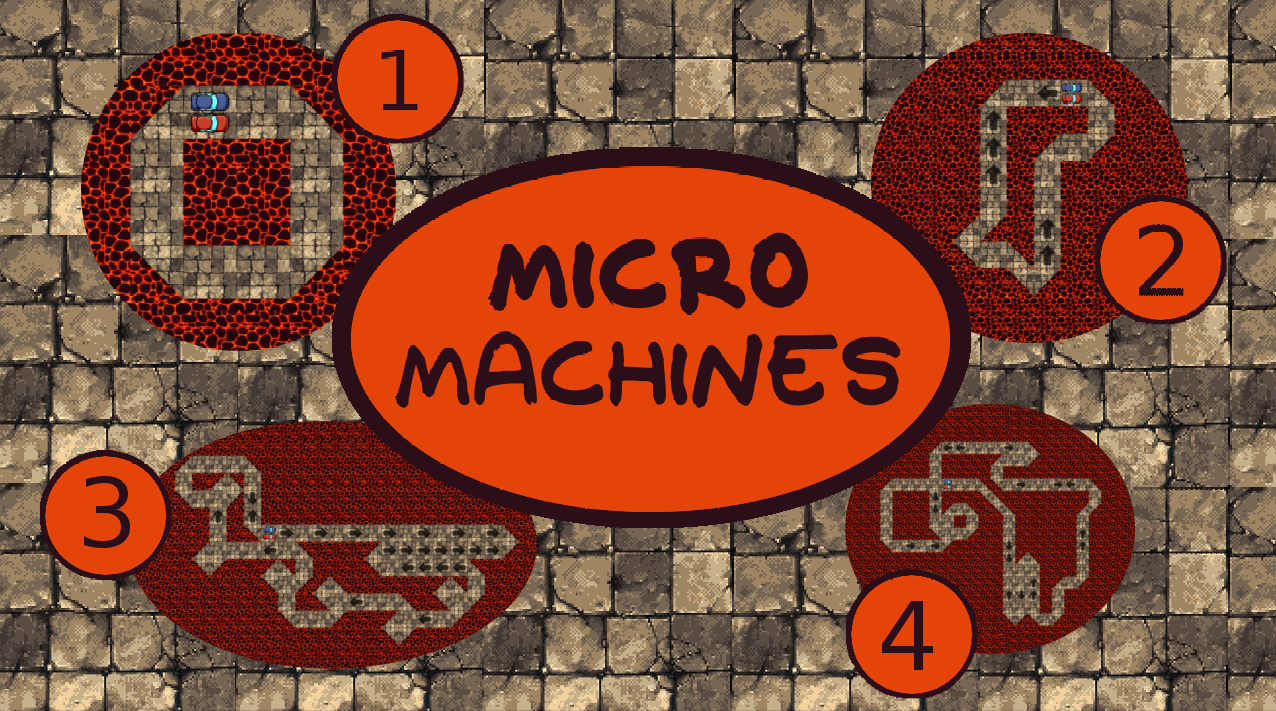
\includegraphics[scale=0.25]{Menu.png}
    \caption{Menu do jogo}
    \label{fig:menu}
\end{figure}

    \item O ecrã em que se escolhe o tipo de circuito;
    
\begin{figure}[H]
    \centering
    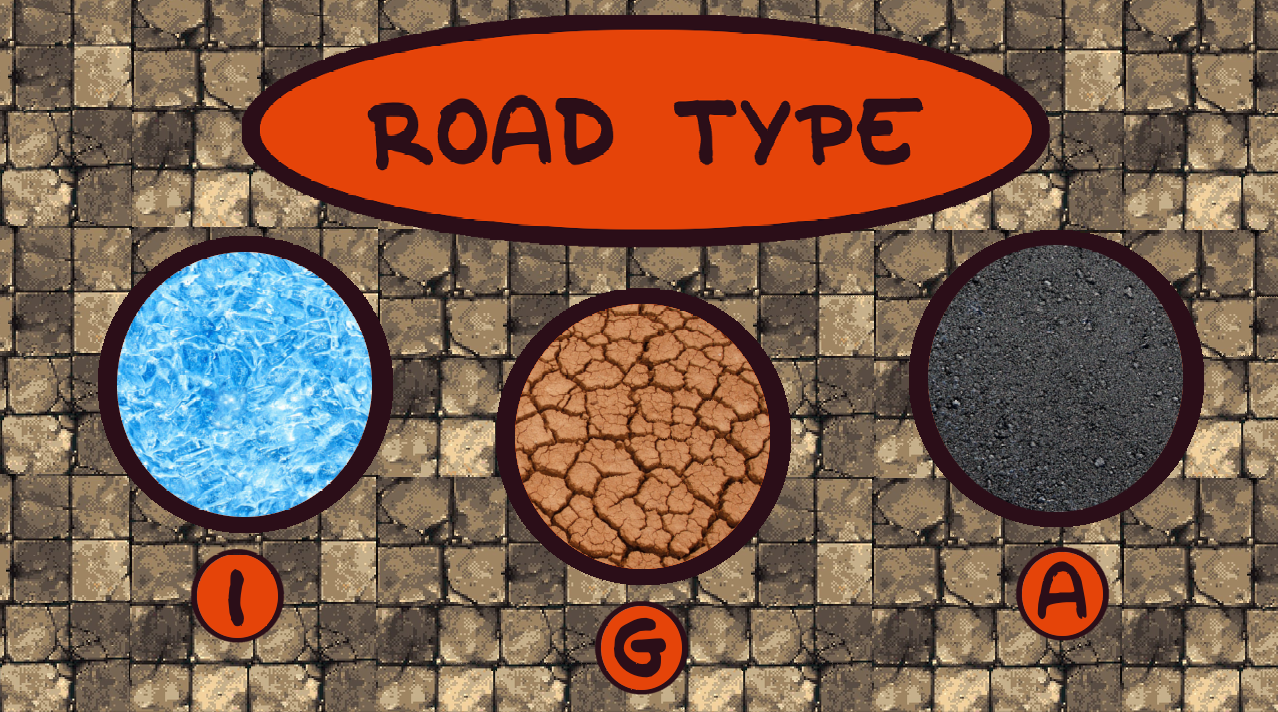
\includegraphics[scale=0.25]{Tipo.png}
    \caption{Ecrã de escolha do tipo de circuito}
    \label{fig:menu}
\end{figure}

    \item O ecrã de pausa;
    
\begin{figure}[H]
    \centering
    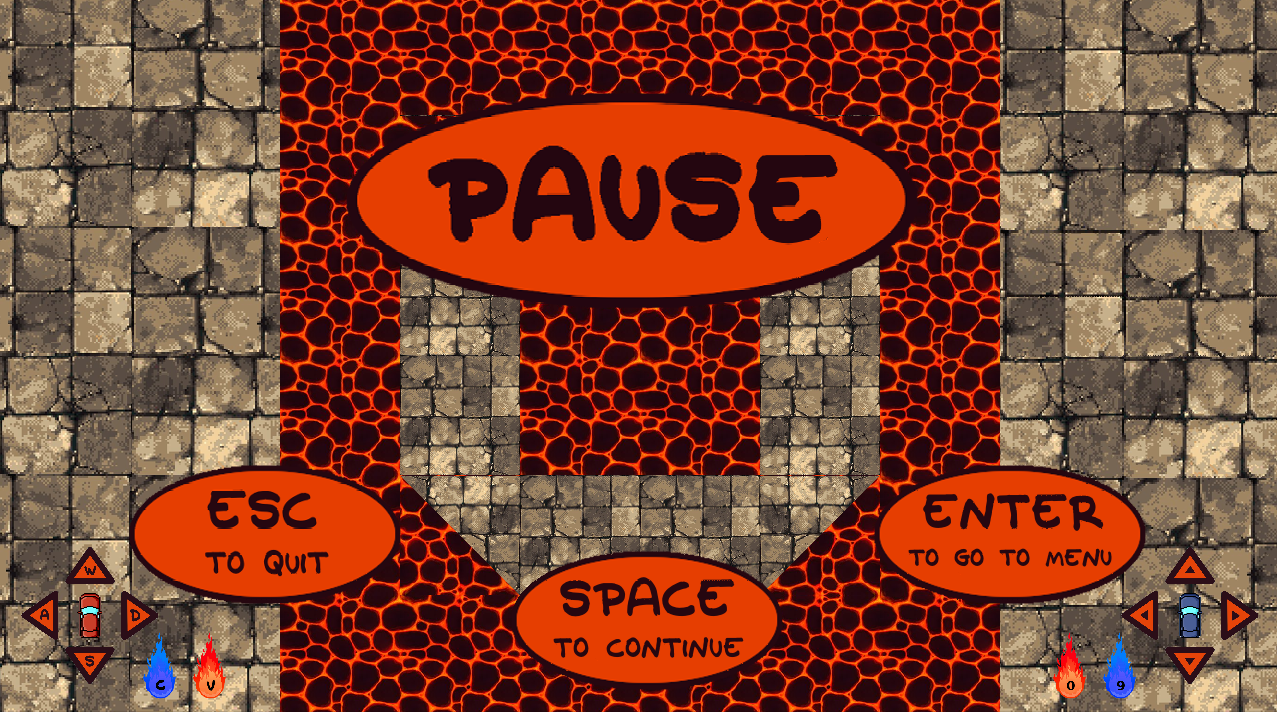
\includegraphics[scale=0.25]{Pausa.png}
    \caption{Ecrã de pausa}
    \label{fig:menu}
\end{figure}

    \item Os ecrãs de vitória;
    
\begin{figure}[H]
    \centering
    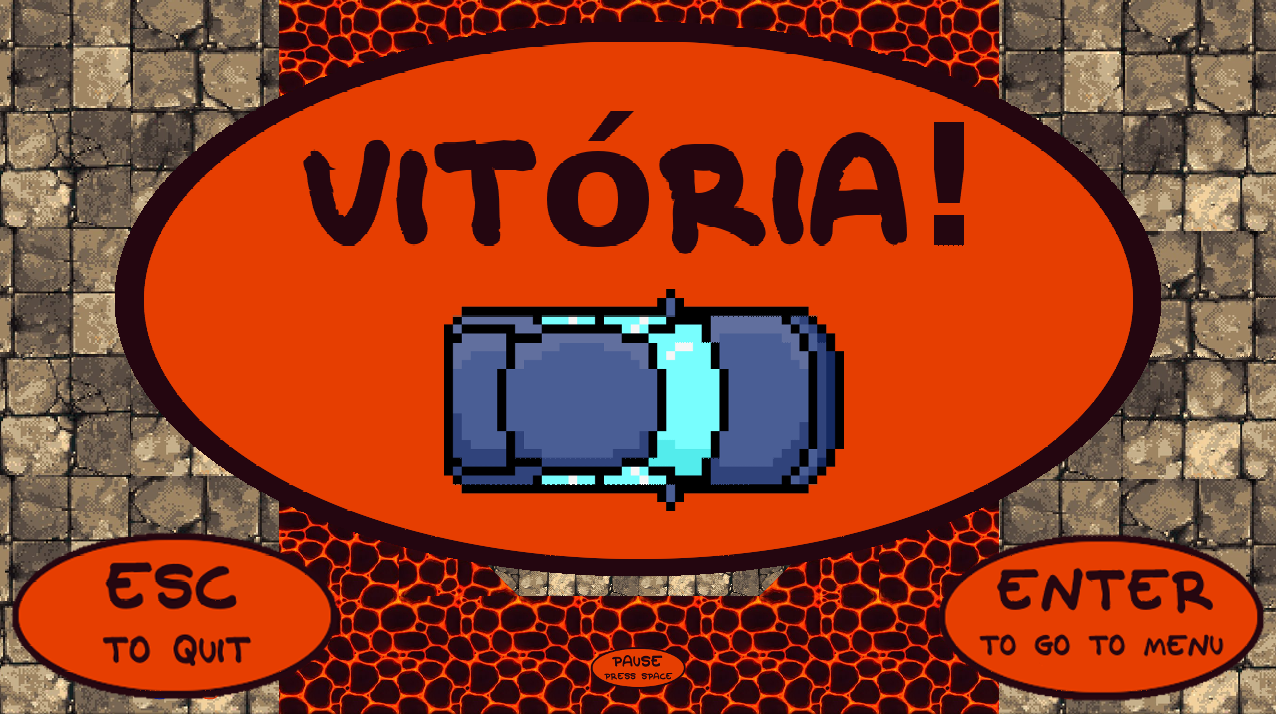
\includegraphics[scale=0.25]{Vitoria.png}
    \caption{Ecrã de vitória}
    \label{fig:menu}
\end{figure}

    \item O jogo em si, com uma interface em que é possível ver todos os controles necessários para o jogar (existem 4 mapas diferentes).
    
\begin{figure}[H]
    \centering
    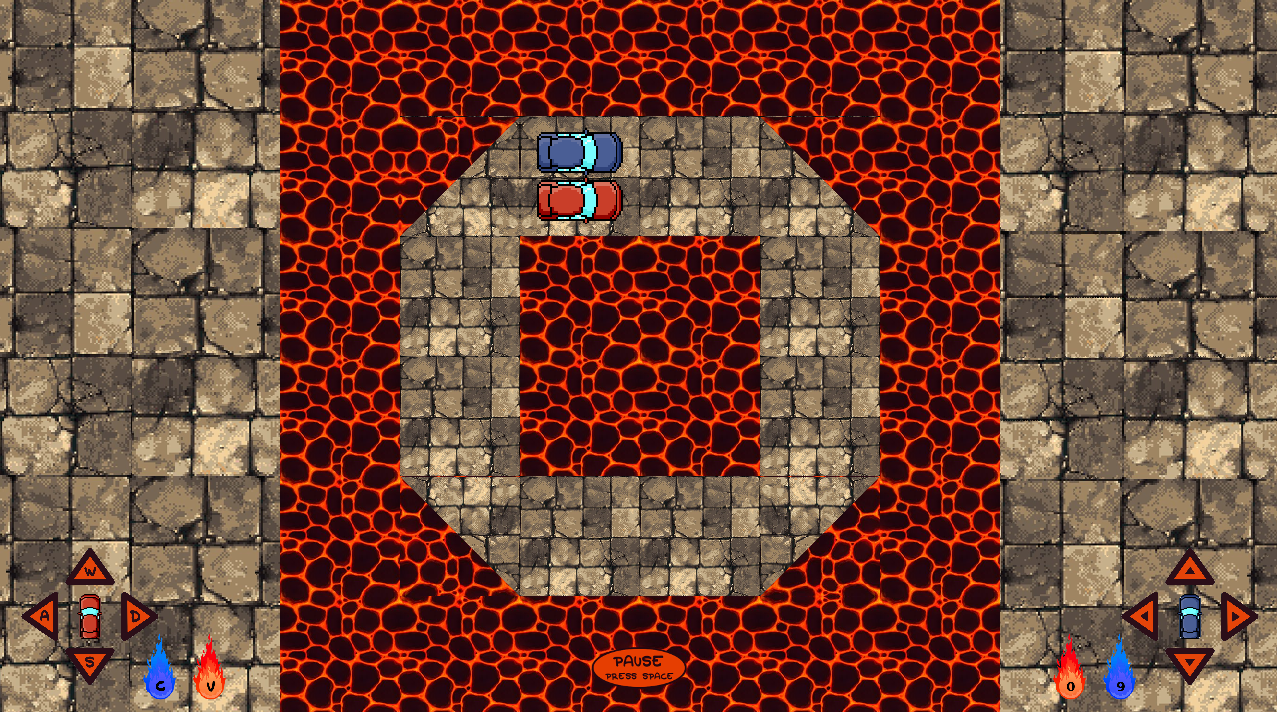
\includegraphics[scale=0.25]{Mapa1.png}
    \caption{Mapa 1}
    \label{fig:menu}
\end{figure}

\begin{figure}[H]
    \centering
    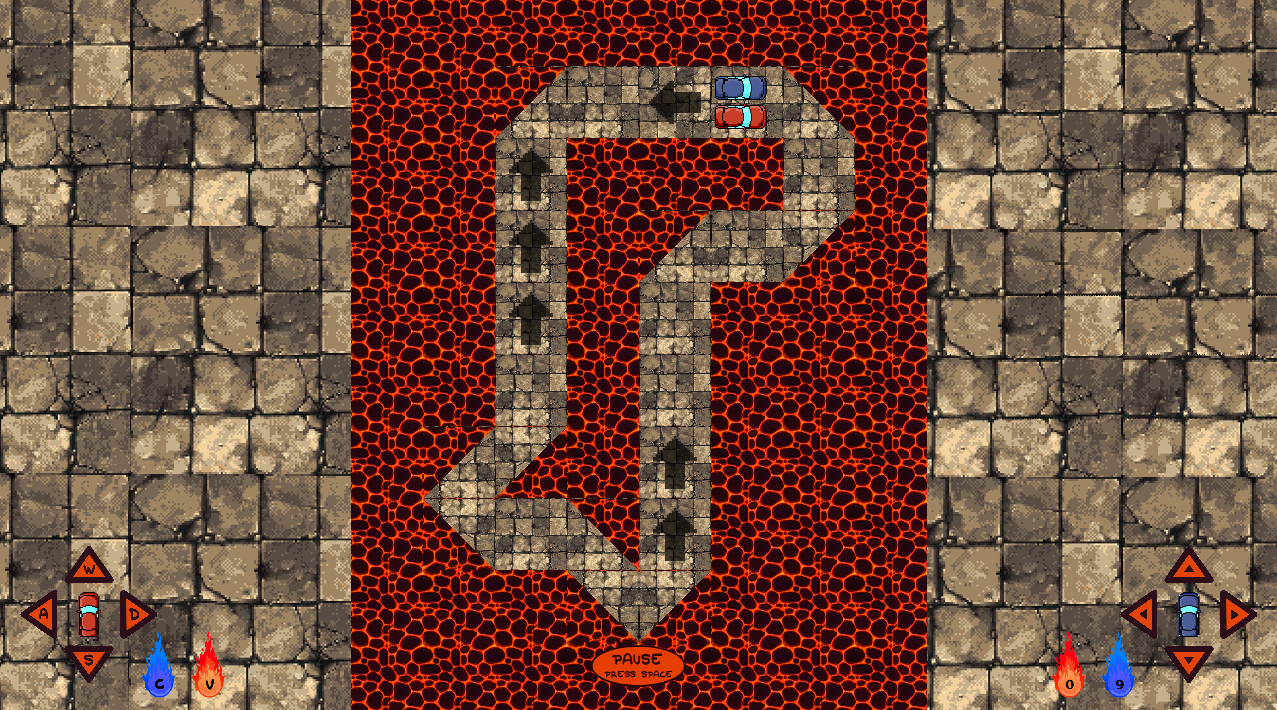
\includegraphics[scale=0.25]{Mapa2.png}
    \caption{Mapa 2}
    \label{fig:menu}
\end{figure}

\begin{figure}[H]
    \centering
    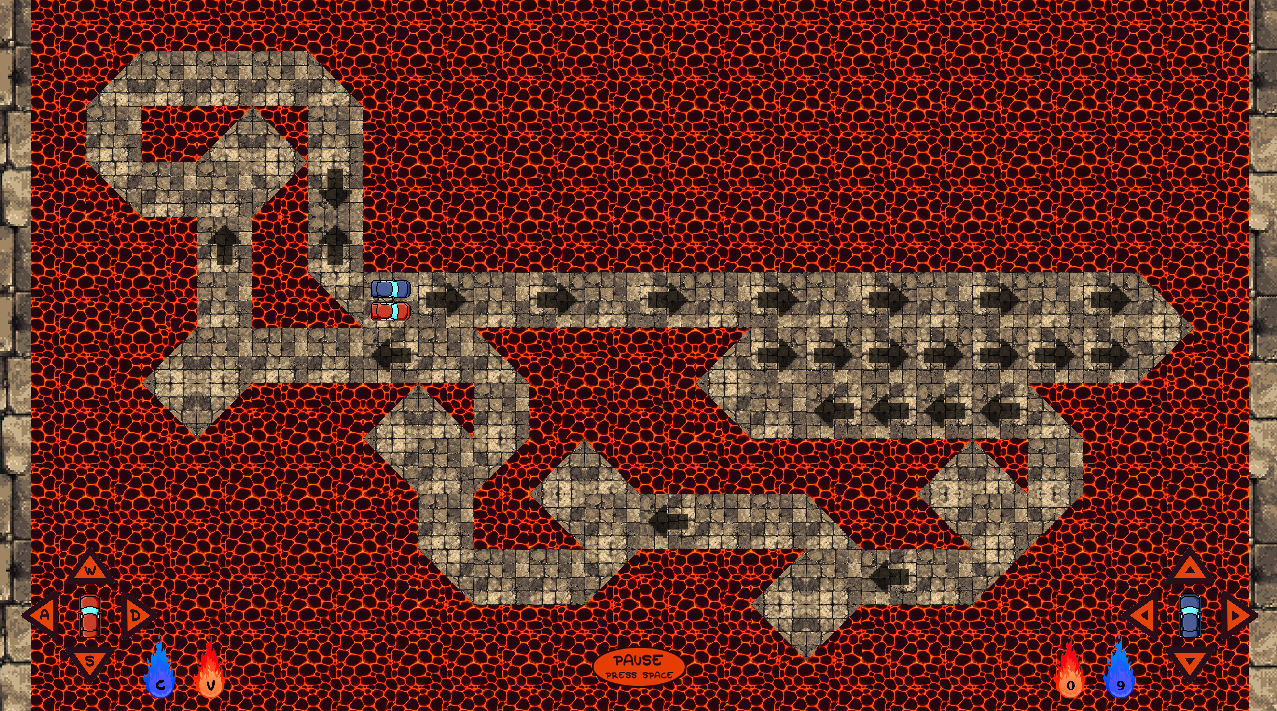
\includegraphics[scale=0.25]{Mapa3.png}
    \caption{Mapa 3}
    \label{fig:menu}
\end{figure}

\begin{figure}[H]
    \centering
    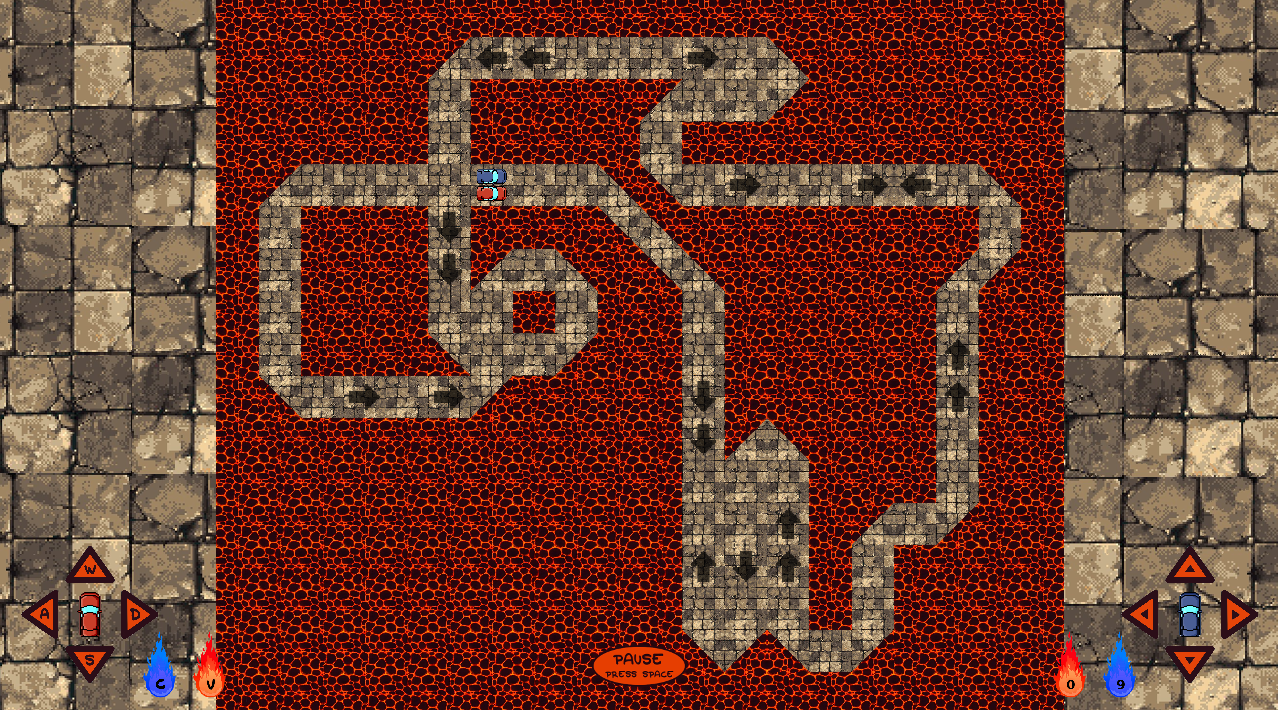
\includegraphics[scale=0.25]{Mapa4.png}
    \caption{Mapa 4}
    \label{fig:menu}
\end{figure}
\end{itemize}

O seguinte parâmetro é a função \textit{reageEvento}, que altera o estado do mundo conforme o \textit{input} dos jogadores. Em geral, há dois tipos de operações que esta função pode levar a cabo:

\begin{itemize}
    \item Alterar as ações no estado do jogo, dependendo das teclas que os jogadores primam enquanto competem.
    \item Alterar os Booleanos no estado do jogo, caso os jogadores não estejam a jogar, propriamente dito. Isto inclui quando estão a escolher o mapa, o tipo de circuito, em pausa ou quando a corrida acaba.
\end{itemize}

Há ainda que notar que quando o jogo é iniciado, dependendo do mapa que o jogador escolher, o mundoInicial vai ser substituído por outro "mundo" que possui todos os dados acerca do mapa escolhido - \textit{mundoInicial1}, \textit{mundoInicial2}, etc. Se os jogadores voltarem a jogar sem sair do programa, o "mundo" será alternado entre estes quatro referidos, não se recuperando o \textit{mundoInicial}.

Por fim, temos a função \textit{reageTempo}, que constitui o último parâmetro recebido pela \textit{play}. Esta é responsável por movimentar o mundo no tempo dado, sendo que vai ser chamada a cada frame (o tempo será, portanto, 1/50 segundos). Esta função pode ser dividida essencialmente em duas partes:

\begin{lstlisting}
reageTempo :: Float -> Mundo -> Mundo
reageTempo n m 
 | menu m = m
 | tipo m = m
 | pausa m = m
 | otherwise = reageTempo2 (float2Double n) (m {jogo = atualiza (float2Double n) (atualiza (float2Double n) (jogo m) 0 (acao0 m)) 1 (acao1 m)})
\end{lstlisting}

A primeira é responsável por atualizar o estado do jogo, recebendo as ações modificadas pela \textit{reageEvento}. Como podemos observar, caso não se esteja a jogar, o mundo é imutável. Caso contrário, é aplicada a função \textit{atualiza}, descrita em \ref{solucaotarefa4}, aos dois carros, atualizando assim as suas direções e velocidades.

Na segunda parte, mais especificamente na função auxiliar, trata-se de atualizar as posições dos carros, recorrendo à tarefa 3. Caso a \textit{movimenta} retorne um \textit{Nothing}, o que significa que o carro é destruído, o carro reaparece no centro da última peça visitada, com velocidade nula. Por fim, é também nesta segunda parte que se verifica se o jogo já acabou, com o auxílio da seguinte função:

\begin{lstlisting}
contaVoltas :: [[Posicao]] -> Tabuleiro -> Bool
contaVoltas [h,t] tab 
  | length h < 2 && length t < 2 = False
  | length h < 2 && length t >= 2 = (head t == last t && t!!1 == (fst(last t)-1,snd(last t))) && length t >= difLava tab
  | length h >= 2 && length t < 2 = (head h == last h && h!!1 == (fst(last h)-1,snd(last h))) && length h >= difLava tab
  | otherwise = ((head h == last h && h!!1 == (fst(last h)-1,snd(last h))) || (head t == last t && t!!1 == (fst(last t)-1,snd(last t)))) && (length h >= difLava tab || length t >= difLava tab)
\end{lstlisting}

Como podemos observar, esta função apenas confirma que a corrida já foi ganha se, simultaneamente:

\begin{itemize}
    \item O primeiro e último elementos do histórico de um dos carros for igual - o último elemento é sempre a posição de partida;
    \item A penúltima posição percorrida (segundo elemento do histórico) por esse carro for uma unidade à esquerda da posição de partida (todos os mapas disponíveis começam com orientação Este)
    \item O comprimento do histórico for, no mínimo, igual ao número de peças não Lava que há no tabuleiro.
\end{itemize}

\subsection{Tarefa 6}

Para esta tarefa é possível desenvolver várias estratégias de corrida diferentes. O objetivo é criar um carro que ande sozinho, sendo capaz de completar o percurso, idealmente em menos de um minuto.

A estratégia desenvolvida começa por fazer o carro avançar, no início da corrida. Com isto, logo na primeira frame, a posição inicial é adicionada ao histórico do carro.

Ao longo de todo o percurso, calcula-se a orientação com que o carro vai sair da peça em que se encontra através da seguinte função:

\begin{verbatim}
oriSaida :: Posicao -- posição atual do carro
         -> Ponto -- posição da peça seguinte
         -> Orientacao -- orientação com que sai da peça
oriSaida (a,b) (x,y) | y == realToFrac(b-1) = Norte
                     | x == realToFrac(a+1) = Este
                     | y == realToFrac(b+1) = Sul
                     | x == realToFrac(a-1) = Oeste
\end{verbatim}

A posição da peça seguinte que, como podemos ver acima, é fornecida à função \texit{oriSaida}, é calculada através da função \textit{oriToPos} através da posição e da orientação atuais do carro. Esta operação é bastante linear, com a salvaguarda de que quando a peça atual é uma curva, o resultado é diferente do usual. Por exemplo, se a orientação for \textit{Este}:

\begin{verbatim}
estePeca :: Peca -> Posicao -> Ponto
estePeca (Peca (Curva Este) _) (x,y)  = (realToFrac x,realToFrac (y+1))
estePeca (Peca (Curva Sul) _) (x,y)   = (realToFrac x,realToFrac (y-1))
estePeca _  (x,y) = (realToFrac (x+1), realToFrac y)
\end{verbatim}

A função acima é uma das quatro funções auxiliares a que a \textit{oriToPos} recorre para calcular a posição da peça seguinte, existindo uma para cada orientação.

Contudo, para saber a orientação atual do carro, que é preciso fornecer à \textit{oriToPos}, é ainda necessário chamar a função \textit{oriEnt}. Esta função calcula a orientação com que o carro entrou na peça atual, verificando as posições relativas das duas últimas peças visitadas pelo carro:

\begin{verbatim}
oriEnt :: Posicao -> Posicao -> Orientacao
oriEnt (a,b) (x,y) | y == b-1 = Norte
                   | x == a+1 = Este
                   | y == b+1 = Sul
                   | x == a-1 = Oeste
\end{verbatim}

Quando o histórico do carro possui apenas uma posição, no início da corrida, não é possível utilizar esta função. Ao revés disso, fornece-se à \textit{oriToPos} a orientação inicial, presente no mapa.

Sabendo a orientação com que o carro vai sair da peça, é então possível gerar uma ação para o carro (que é o objetivo desta tarefa). Assim, define-se a função \textit{direcionar2}, que gera a ação necessária para atualizar a direção do carro conforme a orientação que este tem de tomar para sair da peça.

Sempre que é necessário alterar a direção do carro, o carro trava até parar, roda quando fica estático, virando-se na direção da próxima peça e volta a acelerar de novo. Desta forma, evita-se que o carro saia da peça e seja destruído, o que poderia acontecer se tentasse rodar enquanto acelerava. Caso o circuito tenha as propriedades do tipo gelo, o que se verifica através do k\_roda, o carro vai travando e rodando ao mesmo tempo, de maneira a tentar evitar que o carro deslize.

A função \textit{bot}, com tudo isto, produz uma ação para o carro executar.

\chapter{Validação da Solução}

\section{Fase 1}

\subsection{Tarefa 1}
\label{validacaotarefa1}

Por fim, nesta tarefa, gerou-se um conjunto de testes de maneira a perceber se a solução usada cobria todos os casos possíveis.

Os primeiros cinco testes, que se podem ver abaixo, verificam que o mapa é bem construído independentemente do passo inicial do caminho dado.

\begin{verbatim}
c1 = [Avanca,CurvaEsq,CurvaEsq,Avanca,CurvaEsq,CurvaEsq]
c2 = [Sobe,CurvaEsq,Sobe,CurvaEsq,Sobe,Desce,CurvaEsq,Desce,CurvaEsq,Desce]
c3 = [Desce,CurvaDir,CurvaDir,Sobe,CurvaDir,CurvaDir]
c4 = [CurvaDir,Sobe,CurvaDir,CurvaDir,Desce,CurvaDir]
c5 = [CurvaEsq,CurvaEsq,Avanca,CurvaEsq,CurvaEsq,Avanca]
\end{verbatim}

Como podemos observar, cada um dos cinco caminhos supracitados começa por um passo diferente, cobrindo todas as possibilidades para o passo inicial do caminho.

O teste seguinte descreve um circuito em forma de oito, havendo repetição da posição de duas peças do circuito.

\begin{lstlisting}
c6 = [Sobe,CurvaEsq,Avanca,CurvaDir,Sobe,CurvaDir,CurvaDir,Desce,Avanca,Desce,CurvaEsq,CurvaEsq]
\end{lstlisting}

Neste caso, os passos correspondentes às peças que se sobrepõem são ambos 'Avanca', pelo que as peças correspondentes também vão ser iguais, do tipo Recta. Logo, não se cria qualquer conflito, visto que as peças do tipo Recta não têm orientação, podendo o carro entrar por qualquer lado da peça. Caso as peças que se sobrepõem fossem diferentes, o tabuleiro ficaria mal construído, como se poderia verificar posteriormente na Tarefa 2.

Por fim, o último teste é bastante simples.

\begin{verbatim}
c7 = []
\end{verbatim}

Dado um caminho vazio, é esperado que a função \textit{constroi} devolva um tabuleiro formado apenas por peças do tipo lava. Contudo, apesar da simplicidade deste teste, a função daria erro se não fosse adicionado um caso de paragem à mesma.

\subsection{Tarefa 2}

Cada teste desta tarefa é constituído por um tabuleiro. Desta maneira, procurou-se usar tabuleiros que não verificassem apenas uma das condições, tentando assim percorrer todas as condições uma a uma, e explorar o que podia levá-las a não ser verificadas.

Além disso, não podemos esquecer que, embora os testes sejam tabuleiros, um mapa é constituído pela posição inicial, pela orientação inicial e pelo tabuleiro. Isto justifica a criação o uso da posição \textit{PosTabuleiro}, que verifica se todas as posições do circuito, especialmente a posição inicial do mapa, faz parte do tabuleiro.

O primeiro teste consiste num tabuleiro vazio. É o caso mais simples para um mapa não válido e, sem o caso de paragem na função \textit{valida}, daria um erro de padrões não-exaustivos na mesma.

\begin{verbatim}
t1 = []
valida (Mapa(p,o) []) = False
\end{verbatim}

O segundo teste consiste num tabuleiro que não é rodeado por lava, nomeadamente a sua última fila tem peças não Lava:

\begin{lstlisting}
t2 = [[Peca Lava 0,Peca Lava 0,Peca Lava 0,Peca Lava 0,Peca Lava 0],[Peca Lava 0,Peca (Curva Norte) 0,Peca Recta 0,Peca (Curva Este) 0,Peca Lava 0],[Peca Lava 0,Peca Recta 0,Peca Lava 0,Peca Recta 0,Peca Lava 0],[Peca Lava 0,Peca (Curva Oeste) 0,Peca Recta 0,Peca (Curva Sul) 0,Peca Lava 0]]
\end{lstlisting}

O terceiro teste é um tabuleiro não retangular. A última linha é mais curta que as restantes do tabuleiro:

\begin{lstlisting}
t3 = [[Peca Lava 0,Peca Lava 0,Peca Lava 0,Peca Lava 0,Peca Lava 0],[Peca Lava 0,Peca (Curva Norte) 0,Peca Recta 0,Peca (Curva Este) 0,Peca Lava 0],[Peca Lava 0,Peca Recta 0,Peca Lava 0,Peca Recta 0,Peca Lava 0],[Peca Lava 0,Peca (Curva Oeste) 0,Peca Recta 0,Peca (Curva Sul) 0,Peca Lava 0],[Peca Lava 0,Peca Lava 0,Peca Lava 0,Peca Lava 0]]
\end{lstlisting}

No quarto teste, nem todas as peças Lava estão à altura 0:

\begin{lstlisting}
t4 = [[Peca Lava 0,Peca Lava 0,Peca Lava 1,Peca Lava 0,Peca Lava 0],[Peca Lava 0,Peca (Curva Norte) 0,Peca Recta 0,Peca (Curva Este) 0,Peca Lava 0],[Peca Lava 0,Peca Recta 0,Peca Lava 0,Peca Recta 0,Peca Lava 0],[Peca Lava 0,Peca (Curva Oeste) 0,Peca Recta 0,Peca (Curva Sul) 0,Peca Lava 0],[Peca Lava 0,Peca Lava 0,Peca Lava 0,Peca Lava 0,Peca Lava 0]]
\end{lstlisting}

No seguinte, as peças do percurso não estão ligadas apenas a peças do percurso com alturas compatíveis. Como podemos observar na segunda linha, há uma peça Recta de altura 0 ligada a uma peça Curva de altura 1:

\begin{lstlisting}
t5 = [[Peca Lava 0,Peca Lava 0,Peca Lava 0,Peca Lava 0,Peca Lava 0],[Peca Lava 0,Peca (Curva Norte) 0,Peca Recta 0,Peca (Curva Este) 1,Peca Lava 0],[Peca Lava 0,Peca Recta 0,Peca Lava 0,Peca Recta 0,Peca Lava 0],[Peca Lava 0,Peca (Curva Oeste) 0,Peca Recta 0,Peca (Curva Sul) 0,Peca Lava 0],[Peca Lava 0,Peca Lava 0,Peca Lava 0,Peca Lava 0,Peca Lava 0]]
\end{lstlisting}

O sexto teste não corresponde a uma trajetória, uma vez que o circuito não é fechado, pois partindo-se da peça inicial com a orientação inicial, não se retorna à mesma. Neste caso, o carro acabaria por chegar a um beco sem saída:

\begin{lstlisting}
t6 = [[Peca Lava 0,Peca Lava 0,Peca Lava 0,Peca Lava 0,Peca Lava 0],[Peca Lava 0,Peca (Curva Oeste) 0,Peca Recta 0,Peca (Curva Este) 0,Peca Lava 0],[Peca Lava 0,Peca Recta 0,Peca Lava 0,Peca Recta 0,Peca Lava 0],[Peca Lava 0,Peca (Curva Oeste) 0,Peca Recta 0,Peca (Curva Sul) 0,Peca Lava 0],[Peca Lava 0,Peca Lava 0,Peca Lava 0,Peca Lava 0,Peca Lava 0]]
\end{lstlisting}

O último teste é invalidado porque nem todas as peças fora do percurso são do tipo lava, sendo a última peça do tabuleiro de tipo Recta:

\begin{lstlisting}
t7 = [[Peca Lava 0,Peca Lava 0,Peca Lava 0,Peca Lava 0,Peca Lava 0],[Peca Lava 0,Peca (Curva Norte) 0,Peca Recta 0,Peca (Curva Este) 0,Peca Lava 0],[Peca Lava 0,Peca Recta 0,Peca Lava 0,Peca Recta 0,Peca Lava 0],[Peca Lava 0,Peca (Curva Oeste) 0,Peca Recta 0,Peca (Curva Sul) 0,Peca Lava 0],[Peca Lava 0,Peca Lava 0,Peca Lava 0,Peca Lava 0,Peca Recta 0]]
\end{lstlisting}

\subsection{Tarefa 3}

Ao longo do desenvolvimento da tarefa 3, recorreu-se muito ao simulador de colisões disponibilizado pelos docentes no site de apoio à unidade curricular, de maneira a testar as interações do carro com o mapa, procurando explorar todos os caso possíveis. Por este motivo, a maioria dos testes desta tarefa usam o mesmo mapa que o dito simulador.

Teste 1 - o carro é direcionado para o canto inferior direito da peça atual, sendo que a aparência do mapa deixa dúvidas sobre se o carro deve seguir em frente ou fazer ricochete, dado que depois da peça atual há um encadeamento de curvas:

\begin{lstlisting}
t1 = ([[Peca Lava 0,Peca Lava 0,Peca Lava 0,Peca Lava 0,Peca Lava 0,Peca Lava 0,Peca Lava 0,Peca Lava 0,Peca Lava 0,Peca Lava 0,Peca Lava 0,Peca Lava 0],[Peca Lava 0,Peca Lava 0,Peca Lava 0,Peca Lava 0,Peca (Curva Norte) 0,Peca Recta 0,Peca (Curva Este) 0,Peca Lava 0,Peca Lava 0,Peca Lava 0,Peca Lava 0,Peca Lava 0],[Peca Lava 0,Peca Lava 0,Peca Lava 0,Peca Lava 0,Peca Recta 0,Peca Lava 0,Peca (Rampa Norte) (-1),Peca Lava 0,Peca Lava 0,Peca Lava 0,Peca Lava 0,Peca Lava 0],[Peca Lava 0,Peca (Curva Norte) 0,Peca Recta 0,Peca Recta 0,Peca (Curva Sul) 0,Peca Lava 0,Peca Recta (-1),Peca Lava 0,Peca Lava 0,Peca Lava 0,Peca Lava 0,Peca Lava 0],[Peca Lava 0,Peca Recta 0,Peca Lava 0,Peca Lava 0,Peca Lava 0,Peca Lava 0,Peca (Curva Oeste) (-1),Peca (Curva Este) (-1),Peca Lava 0,Peca Lava 0,Peca Lava 0,Peca Lava 0],[Peca Lava 0,Peca Recta 0,Peca Lava 0,Peca Lava 0,Peca Lava 0,Peca Lava 0,Peca Lava 0,Peca (Curva Oeste) (-1),Peca (Curva Este) (-1),Peca Lava 0,Peca Lava 0,Peca Lava 0],[Peca Lava 0,Peca (Rampa Norte) (-1),Peca Lava 0,Peca Lava 0,Peca Lava 0,Peca Lava 0,Peca Lava 0,Peca (Curva Norte) (-1),Peca (Curva Sul) (-1),Peca Lava 0,Peca Lava 0,Peca Lava 0],[Peca Lava 0,Peca (Rampa Norte) (-2),Peca Lava 0,Peca Lava 0,Peca Lava 0,Peca Lava 0,Peca (Curva Norte) (-1),Peca (Curva Sul) (-1),Peca Lava 0,Peca Lava 0,Peca Lava 0,Peca Lava 0],[Peca Lava 0,Peca (Curva Oeste) (-2),Peca Recta (-2),Peca (Curva Este) (-2),Peca Lava 0,Peca Lava 0,Peca (Curva Oeste) (-1),Peca Recta (-1),Peca Recta (-1),Peca (Rampa Oeste) (-2),Peca (Curva Este) (-2),Peca Lava 0],[Peca Lava 0,Peca Lava 0,Peca Lava 0,Peca (Curva Oeste) (-2),Peca (Curva Este) (-2),Peca Lava 0,Peca (Curva Norte) (-3),Peca (Rampa Este) (-3),Peca Recta (-2),Peca Recta (-2),Peca (Curva Sul) (-2),Peca Lava 0],[Peca Lava 0,Peca Lava 0,Peca Lava 0,Peca Lava 0,Peca (Curva Oeste) (-2),Peca (Rampa Oeste) (-3),Peca (Curva Sul) (-3),Peca Lava 0,Peca Lava 0,Peca Lava 0,Peca Lava 0,Peca Lava 0],[Peca Lava 0,Peca Lava 0,Peca Lava 0,Peca Lava 0,Peca Lava 0,Peca Lava 0,Peca Lava 0,Peca Lava 0,Peca Lava 0,Peca Lava 0,Peca Lava 0,Peca Lava 0]],3,Carro {posicao = (6.5,3.5), direcao = 45, velocidade = (1,1)})
\end{lstlisting}

Teste 2 - o carro faz ricochete na lava e é redirecionado para um canto da nova peça que deixa dúvidas sobre se haverá ricochete ou não, pela aparência:

\begin{lstlisting}
t2 = ([[Peca Lava 0,Peca Lava 0,Peca Lava 0,Peca Lava 0,Peca Lava 0,Peca Lava 0,Peca Lava 0,Peca Lava 0,Peca Lava 0,Peca Lava 0,Peca Lava 0,Peca Lava 0],[Peca Lava 0,Peca Lava 0,Peca Lava 0,Peca Lava 0,Peca (Curva Norte) 0,Peca Recta 0,Peca (Curva Este) 0,Peca Lava 0,Peca Lava 0,Peca Lava 0,Peca Lava 0,Peca Lava 0],[Peca Lava 0,Peca Lava 0,Peca Lava 0,Peca Lava 0,Peca Recta 0,Peca Lava 0,Peca (Rampa Norte) (-1),Peca Lava 0,Peca Lava 0,Peca Lava 0,Peca Lava 0,Peca Lava 0],[Peca Lava 0,Peca (Curva Norte) 0,Peca Recta 0,Peca Recta 0,Peca (Curva Sul) 0,Peca Lava 0,Peca Recta (-1),Peca Lava 0,Peca Lava 0,Peca Lava 0,Peca Lava 0,Peca Lava 0],[Peca Lava 0,Peca Recta 0,Peca Lava 0,Peca Lava 0,Peca Lava 0,Peca Lava 0,Peca (Curva Oeste) (-1),Peca (Curva Este) (-1),Peca Lava 0,Peca Lava 0,Peca Lava 0,Peca Lava 0],[Peca Lava 0,Peca Recta 0,Peca Lava 0,Peca Lava 0,Peca Lava 0,Peca Lava 0,Peca Lava 0,Peca (Curva Oeste) (-1),Peca (Curva Este) (-1),Peca Lava 0,Peca Lava 0,Peca Lava 0],[Peca Lava 0,Peca (Rampa Norte) (-1),Peca Lava 0,Peca Lava 0,Peca Lava 0,Peca Lava 0,Peca Lava 0,Peca (Curva Norte) (-1),Peca (Curva Sul) (-1),Peca Lava 0,Peca Lava 0,Peca Lava 0],[Peca Lava 0,Peca (Rampa Norte) (-2),Peca Lava 0,Peca Lava 0,Peca Lava 0,Peca Lava 0,Peca (Curva Norte) (-1),Peca (Curva Sul) (-1),Peca Lava 0,Peca Lava 0,Peca Lava 0,Peca Lava 0],[Peca Lava 0,Peca (Curva Oeste) (-2),Peca Recta (-2),Peca (Curva Este) (-2),Peca Lava 0,Peca Lava 0,Peca (Curva Oeste) (-1),Peca Recta (-1),Peca Recta (-1),Peca (Rampa Oeste) (-2),Peca (Curva Este) (-2),Peca Lava 0],[Peca Lava 0,Peca Lava 0,Peca Lava 0,Peca (Curva Oeste) (-2),Peca (Curva Este) (-2),Peca Lava 0,Peca (Curva Norte) (-3),Peca (Rampa Este) (-3),Peca Recta (-2),Peca Recta (-2),Peca (Curva Sul) (-2),Peca Lava 0],[Peca Lava 0,Peca Lava 0,Peca Lava 0,Peca Lava 0,Peca (Curva Oeste) (-2),Peca (Rampa Oeste) (-3),Peca (Curva Sul) (-3),Peca Lava 0,Peca Lava 0,Peca Lava 0,Peca Lava 0,Peca Lava 0],[Peca Lava 0,Peca Lava 0,Peca Lava 0,Peca Lava 0,Peca Lava 0,Peca Lava 0,Peca Lava 0,Peca Lava 0,Peca Lava 0,Peca Lava 0,Peca Lava 0,Peca Lava 0]],3,Carro {posicao = (6.5,3.5), direcao = 45, velocidade = (1,-1)})
\end{lstlisting}

Testes 3 e 4 - várias colisões consecutivas:

\begin{lstlisting}
t3 = ([[Peca Lava 0,Peca Lava 0,Peca Lava 0,Peca Lava 0,Peca Lava 0,Peca Lava 0,Peca Lava 0,Peca Lava 0,Peca Lava 0,Peca Lava 0,Peca Lava 0,Peca Lava 0],[Peca Lava 0,Peca Lava 0,Peca Lava 0,Peca Lava 0,Peca (Curva Norte) 0,Peca Recta 0,Peca (Curva Este) 0,Peca Lava 0,Peca Lava 0,Peca Lava 0,Peca Lava 0,Peca Lava 0],[Peca Lava 0,Peca Lava 0,Peca Lava 0,Peca Lava 0,Peca Recta 0,Peca Lava 0,Peca (Rampa Norte) (-1),Peca Lava 0,Peca Lava 0,Peca Lava 0,Peca Lava 0,Peca Lava 0],[Peca Lava 0,Peca (Curva Norte) 0,Peca Recta 0,Peca Recta 0,Peca (Curva Sul) 0,Peca Lava 0,Peca Recta (-1),Peca Lava 0,Peca Lava 0,Peca Lava 0,Peca Lava 0,Peca Lava 0],[Peca Lava 0,Peca Recta 0,Peca Lava 0,Peca Lava 0,Peca Lava 0,Peca Lava 0,Peca (Curva Oeste) (-1),Peca (Curva Este) (-1),Peca Lava 0,Peca Lava 0,Peca Lava 0,Peca Lava 0],[Peca Lava 0,Peca Recta 0,Peca Lava 0,Peca Lava 0,Peca Lava 0,Peca Lava 0,Peca Lava 0,Peca (Curva Oeste) (-1),Peca (Curva Este) (-1),Peca Lava 0,Peca Lava 0,Peca Lava 0],[Peca Lava 0,Peca (Rampa Norte) (-1),Peca Lava 0,Peca Lava 0,Peca Lava 0,Peca Lava 0,Peca Lava 0,Peca (Curva Norte) (-1),Peca (Curva Sul) (-1),Peca Lava 0,Peca Lava 0,Peca Lava 0],[Peca Lava 0,Peca (Rampa Norte) (-2),Peca Lava 0,Peca Lava 0,Peca Lava 0,Peca Lava 0,Peca (Curva Norte) (-1),Peca (Curva Sul) (-1),Peca Lava 0,Peca Lava 0,Peca Lava 0,Peca Lava 0],[Peca Lava 0,Peca (Curva Oeste) (-2),Peca Recta (-2),Peca (Curva Este) (-2),Peca Lava 0,Peca Lava 0,Peca (Curva Oeste) (-1),Peca Recta (-1),Peca Recta (-1),Peca (Rampa Oeste) (-2),Peca (Curva Este) (-2),Peca Lava 0],[Peca Lava 0,Peca Lava 0,Peca Lava 0,Peca (Curva Oeste) (-2),Peca (Curva Este) (-2),Peca Lava 0,Peca (Curva Norte) (-3),Peca (Rampa Este) (-3),Peca Recta (-2),Peca Recta (-2),Peca (Curva Sul) (-2),Peca Lava 0],[Peca Lava 0,Peca Lava 0,Peca Lava 0,Peca Lava 0,Peca (Curva Oeste) (-2),Peca (Rampa Oeste) (-3),Peca (Curva Sul) (-3),Peca Lava 0,Peca Lava 0,Peca Lava 0,Peca Lava 0,Peca Lava 0],[Peca Lava 0,Peca Lava 0,Peca Lava 0,Peca Lava 0,Peca Lava 0,Peca Lava 0,Peca Lava 0,Peca Lava 0,Peca Lava 0,Peca Lava 0,Peca Lava 0,Peca Lava 0]],15,Carro {posicao = (6.8,3.3), direcao = 45, velocidade = (0.5,1)})

t4 = ([[Peca Lava 0,Peca Lava 0,Peca Lava 0,Peca Lava 0,Peca Lava 0,Peca Lava 0,Peca Lava 0,Peca Lava 0,Peca Lava 0,Peca Lava 0,Peca Lava 0,Peca Lava 0],[Peca Lava 0,Peca Lava 0,Peca Lava 0,Peca Lava 0,Peca (Curva Norte) 0,Peca Recta 0,Peca (Curva Este) 0,Peca Lava 0,Peca Lava 0,Peca Lava 0,Peca Lava 0,Peca Lava 0],[Peca Lava 0,Peca Lava 0,Peca Lava 0,Peca Lava 0,Peca Recta 0,Peca Lava 0,Peca (Rampa Norte) (-1),Peca Lava 0,Peca Lava 0,Peca Lava 0,Peca Lava 0,Peca Lava 0],[Peca Lava 0,Peca (Curva Norte) 0,Peca Recta 0,Peca Recta 0,Peca (Curva Sul) 0,Peca Lava 0,Peca Recta (-1),Peca Lava 0,Peca Lava 0,Peca Lava 0,Peca Lava 0,Peca Lava 0],[Peca Lava 0,Peca Recta 0,Peca Lava 0,Peca Lava 0,Peca Lava 0,Peca Lava 0,Peca (Curva Oeste) (-1),Peca (Curva Este) (-1),Peca Lava 0,Peca Lava 0,Peca Lava 0,Peca Lava 0],[Peca Lava 0,Peca Recta 0,Peca Lava 0,Peca Lava 0,Peca Lava 0,Peca Lava 0,Peca Lava 0,Peca (Curva Oeste) (-1),Peca (Curva Este) (-1),Peca Lava 0,Peca Lava 0,Peca Lava 0],[Peca Lava 0,Peca (Rampa Norte) (-1),Peca Lava 0,Peca Lava 0,Peca Lava 0,Peca Lava 0,Peca Lava 0,Peca (Curva Norte) (-1),Peca (Curva Sul) (-1),Peca Lava 0,Peca Lava 0,Peca Lava 0],[Peca Lava 0,Peca (Rampa Norte) (-2),Peca Lava 0,Peca Lava 0,Peca Lava 0,Peca Lava 0,Peca (Curva Norte) (-1),Peca (Curva Sul) (-1),Peca Lava 0,Peca Lava 0,Peca Lava 0,Peca Lava 0],[Peca Lava 0,Peca (Curva Oeste) (-2),Peca Recta (-2),Peca (Curva Este) (-2),Peca Lava 0,Peca Lava 0,Peca (Curva Oeste) (-1),Peca Recta (-1),Peca Recta (-1),Peca (Rampa Oeste) (-2),Peca (Curva Este) (-2),Peca Lava 0],[Peca Lava 0,Peca Lava 0,Peca Lava 0,Peca (Curva Oeste) (-2),Peca (Curva Este) (-2),Peca Lava 0,Peca (Curva Norte) (-3),Peca (Rampa Este) (-3),Peca Recta (-2),Peca Recta (-2),Peca (Curva Sul) (-2),Peca Lava 0],[Peca Lava 0,Peca Lava 0,Peca Lava 0,Peca Lava 0,Peca (Curva Oeste) (-2),Peca (Rampa Oeste) (-3),Peca (Curva Sul) (-3),Peca Lava 0,Peca Lava 0,Peca Lava 0,Peca Lava 0,Peca Lava 0],[Peca Lava 0,Peca Lava 0,Peca Lava 0,Peca Lava 0,Peca Lava 0,Peca Lava 0,Peca Lava 0,Peca Lava 0,Peca Lava 0,Peca Lava 0,Peca Lava 0,Peca Lava 0]],15,Carro {posicao = (6.8,3.3), direcao = 45, velocidade = (0.18,1)})
\end{lstlisting}

Teste 5 - O carro faz ricochete no início de um rampa e dirige-se a um canto de aspeto duvidoso:

\begin{lstlisting}
t5 = ([[Peca Lava 0,Peca Lava 0,Peca Lava 0,Peca Lava 0,Peca Lava 0,Peca Lava 0,Peca Lava 0,Peca Lava 0,Peca Lava 0,Peca Lava 0,Peca Lava 0,Peca Lava 0],[Peca Lava 0,Peca Lava 0,Peca Lava 0,Peca Lava 0,Peca (Curva Norte) 0,Peca Recta 0,Peca (Curva Este) 0,Peca Lava 0,Peca Lava 0,Peca Lava 0,Peca Lava 0,Peca Lava 0],[Peca Lava 0,Peca Lava 0,Peca Lava 0,Peca Lava 0,Peca Recta 0,Peca Lava 0,Peca (Rampa Norte) (-1),Peca Lava 0,Peca Lava 0,Peca Lava 0,Peca Lava 0,Peca Lava 0],[Peca Lava 0,Peca (Curva Norte) 0,Peca Recta 0,Peca Recta 0,Peca (Curva Sul) 0,Peca Lava 0,Peca Recta (-1),Peca Lava 0,Peca Lava 0,Peca Lava 0,Peca Lava 0,Peca Lava 0],[Peca Lava 0,Peca Recta 0,Peca Lava 0,Peca Lava 0,Peca Lava 0,Peca Lava 0,Peca (Curva Oeste) (-1),Peca (Curva Este) (-1),Peca Lava 0,Peca Lava 0,Peca Lava 0,Peca Lava 0],[Peca Lava 0,Peca Recta 0,Peca Lava 0,Peca Lava 0,Peca Lava 0,Peca Lava 0,Peca Lava 0,Peca (Curva Oeste) (-1),Peca (Curva Este) (-1),Peca Lava 0,Peca Lava 0,Peca Lava 0],[Peca Lava 0,Peca (Rampa Norte) (-1),Peca Lava 0,Peca Lava 0,Peca Lava 0,Peca Lava 0,Peca Lava 0,Peca (Curva Norte) (-1),Peca (Curva Sul) (-1),Peca Lava 0,Peca Lava 0,Peca Lava 0],[Peca Lava 0,Peca (Rampa Norte) (-2),Peca Lava 0,Peca Lava 0,Peca Lava 0,Peca Lava 0,Peca (Curva Norte) (-1),Peca (Curva Sul) (-1),Peca Lava 0,Peca Lava 0,Peca Lava 0,Peca Lava 0],[Peca Lava 0,Peca (Curva Oeste) (-2),Peca Recta (-2),Peca (Curva Este) (-2),Peca Lava 0,Peca Lava 0,Peca (Curva Oeste) (-1),Peca Recta (-1),Peca Recta (-1),Peca (Rampa Oeste) (-2),Peca (Curva Este) (-2),Peca Lava 0],[Peca Lava 0,Peca Lava 0,Peca Lava 0,Peca (Curva Oeste) (-2),Peca (Curva Este) (-2),Peca Lava 0,Peca (Curva Norte) (-3),Peca (Rampa Este) (-3),Peca Recta (-2),Peca Recta (-2),Peca (Curva Sul) (-2),Peca Lava 0],[Peca Lava 0,Peca Lava 0,Peca Lava 0,Peca Lava 0,Peca (Curva Oeste) (-2),Peca (Rampa Oeste) (-3),Peca (Curva Sul) (-3),Peca Lava 0,Peca Lava 0,Peca Lava 0,Peca Lava 0,Peca Lava 0],[Peca Lava 0,Peca Lava 0,Peca Lava 0,Peca Lava 0,Peca Lava 0,Peca Lava 0,Peca Lava 0,Peca Lava 0,Peca Lava 0,Peca Lava 0,Peca Lava 0,Peca Lava 0]],2,Carro {posicao = (6.5,3.5), direcao = 45, velocidade = (-1,-1)})
\end{lstlisting}

Teste 6 - inúmeras colisões seguidas em movimento horizontal apenas:

\begin{lstlisting}
t6 = ([[Peca Lava 0,Peca Lava 0,Peca Lava 0,Peca Lava 0,Peca Lava 0,Peca Lava 0,Peca Lava 0,Peca Lava 0,Peca Lava 0,Peca Lava 0,Peca Lava 0,Peca Lava 0],[Peca Lava 0,Peca Lava 0,Peca Lava 0,Peca Lava 0,Peca (Curva Norte) 0,Peca Recta 0,Peca (Curva Este) 0,Peca Lava 0,Peca Lava 0,Peca Lava 0,Peca Lava 0,Peca Lava 0],[Peca Lava 0,Peca Lava 0,Peca Lava 0,Peca Lava 0,Peca Recta 0,Peca Lava 0,Peca (Rampa Norte) (-1),Peca Lava 0,Peca Lava 0,Peca Lava 0,Peca Lava 0,Peca Lava 0],[Peca Lava 0,Peca (Curva Norte) 0,Peca Recta 0,Peca Recta 0,Peca (Curva Sul) 0,Peca Lava 0,Peca Recta (-1),Peca Lava 0,Peca Lava 0,Peca Lava 0,Peca Lava 0,Peca Lava 0],[Peca Lava 0,Peca Recta 0,Peca Lava 0,Peca Lava 0,Peca Lava 0,Peca Lava 0,Peca (Curva Oeste) (-1),Peca (Curva Este) (-1),Peca Lava 0,Peca Lava 0,Peca Lava 0,Peca Lava 0],[Peca Lava 0,Peca Recta 0,Peca Lava 0,Peca Lava 0,Peca Lava 0,Peca Lava 0,Peca Lava 0,Peca (Curva Oeste) (-1),Peca (Curva Este) (-1),Peca Lava 0,Peca Lava 0,Peca Lava 0],[Peca Lava 0,Peca (Rampa Norte) (-1),Peca Lava 0,Peca Lava 0,Peca Lava 0,Peca Lava 0,Peca Lava 0,Peca (Curva Norte) (-1),Peca (Curva Sul) (-1),Peca Lava 0,Peca Lava 0,Peca Lava 0],[Peca Lava 0,Peca (Rampa Norte) (-2),Peca Lava 0,Peca Lava 0,Peca Lava 0,Peca Lava 0,Peca (Curva Norte) (-1),Peca (Curva Sul) (-1),Peca Lava 0,Peca Lava 0,Peca Lava 0,Peca Lava 0],[Peca Lava 0,Peca (Curva Oeste) (-2),Peca Recta (-2),Peca (Curva Este) (-2),Peca Lava 0,Peca Lava 0,Peca (Curva Oeste) (-1),Peca Recta (-1),Peca Recta (-1),Peca (Rampa Oeste) (-2),Peca (Curva Este) (-2),Peca Lava 0],[Peca Lava 0,Peca Lava 0,Peca Lava 0,Peca (Curva Oeste) (-2),Peca (Curva Este) (-2),Peca Lava 0,Peca (Curva Norte) (-3),Peca (Rampa Este) (-3),Peca Recta (-2),Peca Recta (-2),Peca (Curva Sul) (-2),Peca Lava 0],[Peca Lava 0,Peca Lava 0,Peca Lava 0,Peca Lava 0,Peca (Curva Oeste) (-2),Peca (Rampa Oeste) (-3),Peca (Curva Sul) (-3),Peca Lava 0,Peca Lava 0,Peca Lava 0,Peca Lava 0,Peca Lava 0],[Peca Lava 0,Peca Lava 0,Peca Lava 0,Peca Lava 0,Peca Lava 0,Peca Lava 0,Peca Lava 0,Peca Lava 0,Peca Lava 0,Peca Lava 0,Peca Lava 0,Peca Lava 0]],30,Carro {posicao = (6.5,3.5), direcao = 45, velocidade = (-1,0)})
\end{lstlisting}

Teste 7 - o carro dirige-se ao canto de uma peça, cujo aspeto deixa dúvidas acerca de como será o ricochete:

\begin{lstlisting}
t7 = ([[Peca Lava 0,Peca Lava 0,Peca Lava 0,Peca Lava 0,Peca Lava 0,Peca Lava 0,Peca Lava 0,Peca Lava 0,Peca Lava 0,Peca Lava 0,Peca Lava 0,Peca Lava 0],[Peca Lava 0,Peca Lava 0,Peca Lava 0,Peca Lava 0,Peca (Curva Norte) 0,Peca Recta 0,Peca (Curva Este) 0,Peca Lava 0,Peca Lava 0,Peca Lava 0,Peca Lava 0,Peca Lava 0],[Peca Lava 0,Peca Lava 0,Peca Lava 0,Peca Lava 0,Peca Recta 0,Peca Lava 0,Peca (Rampa Norte) (-1),Peca Lava 0,Peca Lava 0,Peca Lava 0,Peca Lava 0,Peca Lava 0],[Peca Lava 0,Peca (Curva Norte) 0,Peca Recta 0,Peca Recta 0,Peca (Curva Sul) 0,Peca Lava 0,Peca Recta (-1),Peca Lava 0,Peca Lava 0,Peca Lava 0,Peca Lava 0,Peca Lava 0],[Peca Lava 0,Peca Recta 0,Peca Lava 0,Peca Lava 0,Peca Lava 0,Peca Lava 0,Peca (Curva Oeste) (-1),Peca (Curva Este) (-1),Peca Lava 0,Peca Lava 0,Peca Lava 0,Peca Lava 0],[Peca Lava 0,Peca Recta 0,Peca Lava 0,Peca Lava 0,Peca Lava 0,Peca Lava 0,Peca Lava 0,Peca (Curva Oeste) (-1),Peca (Curva Este) (-1),Peca Lava 0,Peca Lava 0,Peca Lava 0],[Peca Lava 0,Peca (Rampa Norte) (-1),Peca Lava 0,Peca Lava 0,Peca Lava 0,Peca Lava 0,Peca Lava 0,Peca (Curva Norte) (-1),Peca (Curva Sul) (-1),Peca Lava 0,Peca Lava 0,Peca Lava 0],[Peca Lava 0,Peca (Rampa Norte) (-2),Peca Lava 0,Peca Lava 0,Peca Lava 0,Peca Lava 0,Peca (Curva Norte) (-1),Peca (Curva Sul) (-1),Peca Lava 0,Peca Lava 0,Peca Lava 0,Peca Lava 0],[Peca Lava 0,Peca (Curva Oeste) (-2),Peca Recta (-2),Peca (Curva Este) (-2),Peca Lava 0,Peca Lava 0,Peca (Curva Oeste) (-1),Peca Recta (-1),Peca Recta (-1),Peca (Rampa Oeste) (-2),Peca (Curva Este) (-2),Peca Lava 0],[Peca Lava 0,Peca Lava 0,Peca Lava 0,Peca (Curva Oeste) (-2),Peca (Curva Este) (-2),Peca Lava 0,Peca (Curva Norte) (-3),Peca (Rampa Este) (-3),Peca Recta (-2),Peca Recta (-2),Peca (Curva Sul) (-2),Peca Lava 0],[Peca Lava 0,Peca Lava 0,Peca Lava 0,Peca Lava 0,Peca (Curva Oeste) (-2),Peca (Rampa Oeste) (-3),Peca (Curva Sul) (-3),Peca Lava 0,Peca Lava 0,Peca Lava 0,Peca Lava 0,Peca Lava 0],[Peca Lava 0,Peca Lava 0,Peca Lava 0,Peca Lava 0,Peca Lava 0,Peca Lava 0,Peca Lava 0,Peca Lava 0,Peca Lava 0,Peca Lava 0,Peca Lava 0,Peca Lava 0]],5,Carro {posicao = (6.5,3.5), direcao = 45, velocidade = (-1,1)})
\end{lstlisting}

Teste 8 - o carro está numa rampa ascendente e dirige-se a outra rampa, com a qual não deve colidir, mas sim transitar para ela normalmente, porque a diferença das alturas naquele ponto é inferior a uma unidade:

\begin{lstlisting}
t8 = ([[Peca Lava 0,Peca Lava 0,Peca Lava 0,Peca Lava 0,Peca Lava 0,Peca Lava 0,Peca Lava 0],[Peca Lava 0,Peca (Curva Norte) 1,Peca (Rampa Oeste) 0,Peca (Rampa Este) 0,Peca (Rampa Oeste) 0,Peca (Curva Este) 0,Peca Lava 0],[Peca Lava 0,Peca (Curva Oeste) 1,Peca Recta 1,Peca (Rampa Oeste) 0,Peca Recta 0,Peca (Curva Sul) 0,Peca Lava 0],[Peca Lava 0,Peca Lava 0,Peca Lava 0,Peca Lava 0,Peca Lava 0,Peca Lava 0,Peca Lava 0]],3,Carro {posicao = (3.8,2.5), direcao = 45, velocidade = (-1.4,-1)})
\end{lstlisting}

Teste 9 - outro caso duvidoso com rampas, semelhante ao anterior:

\begin{lstlisting}
t9 = ([[Peca Lava 0,Peca Lava 0,Peca Lava 0,Peca Lava 0,Peca Lava 0,Peca Lava 0,Peca Lava 0],[Peca Lava 0,Peca (Curva Norte) 1,Peca (Rampa Oeste) 0,Peca (Rampa Este) 0,Peca (Rampa Oeste) 0,Peca (Curva Este) 0,Peca Lava 0],[Peca Lava 0,Peca (Curva Oeste) 1,Peca Recta 1,Peca (Rampa Oeste) 0,Peca Recta 0,Peca (Curva Sul) 0,Peca Lava 0],[Peca Lava 0,Peca Lava 0,Peca Lava 0,Peca Lava 0,Peca Lava 0,Peca Lava 0,Peca Lava 0]],3,Carro {posicao = (3.8,2.5), direcao = 45, velocidade = (0,-1)})
\end{lstlisting}

Teste 10 - ricochete com lava numa rampa:

\begin{lstlisting}
t10 = ([[Peca Lava 0,Peca Lava 0,Peca Lava 0,Peca Lava 0,Peca Lava 0,Peca Lava 0,Peca Lava 0],[Peca Lava 0,Peca (Curva Norte) 0,Peca (Rampa Oeste) (-1),Peca (Rampa Este) (-1),Peca (Rampa Oeste) (-1),Peca (Curva Este) (-1),Peca Lava 0],[Peca Lava 0,Peca (Curva Oeste) 0,Peca Recta 0,Peca (Rampa Oeste) (-1),Peca Recta (-1),Peca (Curva Sul) (-1),Peca Lava 0],[Peca Lava 0,Peca Lava 0,Peca Lava 0,Peca Lava 0,Peca Lava 0,Peca Lava 0,Peca Lava 0]] ,4,Carro {posicao = (4.8,1.2), direcao = 45, velocidade = (1,0.5)})
\end{lstlisting}

Teste 11 - o carro faz ricochetes, eventualmente começando a andar para trás no percurso:

\begin{lstlisting}
t11 = ([[Peca Lava 0,Peca Lava 0,Peca Lava 0,Peca Lava 0,Peca Lava 0,Peca Lava 0,Peca Lava 0],[Peca Lava 0,Peca (Curva Norte) 0,Peca (Rampa Oeste) (-1),Peca (Rampa Este) (-1),Peca (Rampa Oeste) (-1),Peca (Curva Este) (-1),Peca Lava 0],[Peca Lava 0,Peca (Curva Oeste) 0,Peca Recta 0,Peca (Rampa Oeste) (-1),Peca Recta (-1),Peca (Curva Sul) (-1),Peca Lava 0],[Peca Lava 0,Peca Lava 0,Peca Lava 0,Peca Lava 0,Peca Lava 0,Peca Lava 0,Peca Lava 0]],8,Carro {posicao = (4.8,1.2), direcao = 45, velocidade = (1,0.159)})
\end{lstlisting}

\section{Fase 2}

\subsection{Tarefa 4}

Para validar a Tarefa 4, fez-se por criar testes que cobrissem o maior número de ações diferentes possível, a fim de testar as interações entre as várias forças e, principalmente, para testar a aplicabilidade da função que aplica o k\_pneus, que foi a função mais problemática ao longo do desenvolvimento desta tarefa.

Como todos os testes são todos do mesmo género e pouco muda de uns para outros, de seguida vai-se apenas dizer sinteticamente o propósito de cada um, isto é, o que se procura explorar com cada teste:

Teste 1 - capacidade de rodagem do carro para a esquerda:

\begin{lstlisting}
t1 = (1,Jogo { mapa  = Mapa ((2,1),Este) [[Peca Lava 0,Peca Lava 0,Peca Lava 0,Peca Lava 0,Peca Lava 0],[Peca Lava 0,Peca (Curva Norte) 0,Peca Recta 0,Peca (Curva Este) 0,Peca Lava 0],[Peca Lava 0,Peca (Rampa Sul) 0,Peca Lava 0,Peca (Rampa Sul) 0,Peca Lava 0],[Peca Lava 0,Peca (Curva Oeste) 1,Peca Recta 1,Peca (Curva Sul) 1,Peca Lava 0],[Peca Lava 0,Peca Lava 0,Peca Lava 0,Peca Lava 0,Peca Lava 0]], pista = Propriedades { k_atrito  = 0, k_pneus = 0.5, k_acel = 4, k_peso = 2, k_nitro = 15, k_roda = 180}, carros = [Carro {posicao = (2.01,1.01), direcao = 45, velocidade = (0.9,0.9)}], nitros  = [5] , historico  = [[]] },Acao { acelerar = False, travar  = False , esquerda = True, direita  = False, nitro  = Nothing })
\end{lstlisting}

Teste 2 - força de aceleração do nitro, força de atrito e força dos pneus:

\begin{lstlisting}
t2 = (0.5,Jogo { mapa  = Mapa ((2,1),Este) [[Peca Lava 0,Peca Lava 0,Peca Lava 0,Peca Lava 0,Peca Lava 0],[Peca Lava 0,Peca (Curva Norte) 0,Peca Recta 0,Peca (Curva Este) 0,Peca Lava 0],[Peca Lava 0,Peca (Rampa Sul) 0,Peca Lava 0,Peca (Rampa Sul) 0,Peca Lava 0],[Peca Lava 0,Peca (Curva Oeste) 1,Peca Recta 1,Peca (Curva Sul) 1,Peca Lava 0],[Peca Lava 0,Peca Lava 0,Peca Lava 0,Peca Lava 0,Peca Lava 0]], pista = Propriedades { k_atrito  = 0.5, k_pneus = 0.5, k_acel = 0.5, k_peso = 2, k_nitro = 2, k_roda = 180}, carros = [Carro {posicao = (2,1.50), direcao = 405, velocidade = (1,0)}], nitros  = [5] , historico  = [[]] },Acao { acelerar = False, travar  = False , esquerda = False, direita  = False, nitro  = Just 0 })
\end{lstlisting}

Teste 3 - força do peso (o carro encontra-se numa rampa);

Teste 4 - força de aceleração do nitro;

Testes 3, 4 e 5 - ângulos do atrito (k\_pneus):

\begin{lstlisting}
t3 = (0.5,Jogo { mapa  = Mapa ((2,1),Este) [[Peca Lava 0,Peca Lava 0,Peca Lava 0,Peca Lava 0,Peca Lava 0],[Peca Lava 0,Peca (Curva Norte) 0,Peca Recta 0,Peca (Curva Este) 0,Peca Lava 0],[Peca Lava 0,Peca (Rampa Sul) 0,Peca Lava 0,Peca (Rampa Sul) 0,Peca Lava 0],[Peca Lava 0,Peca (Curva Oeste) 1,Peca Recta 1,Peca (Curva Sul) 1,Peca Lava 0],[Peca Lava 0,Peca Lava 0,Peca Lava 0,Peca Lava 0,Peca Lava 0]], pista = Propriedades { k_atrito  = 0.5, k_pneus = 0.5, k_acel = 0.5, k_peso = 2, k_nitro = 2, k_roda = 180}, carros = [Carro {posicao = (3.5,2.01), direcao = -360, velocidade = (0,1)}], nitros  = [5] , historico  = [[]] },Acao { acelerar = False, travar  = False , esquerda = False, direita  = False, nitro  = Nothing })

t4 = (0.5,Jogo { mapa  = Mapa ((2,1),Este) [[Peca Lava 0,Peca Lava 0,Peca Lava 0,Peca Lava 0,Peca Lava 0],[Peca Lava 0,Peca (Curva Norte) 0,Peca Recta 0,Peca (Curva Este) 0,Peca Lava 0],[Peca Lava 0,Peca (Rampa Sul) 0,Peca Lava 0,Peca (Rampa Sul) 0,Peca Lava 0],[Peca Lava 0,Peca (Curva Oeste) 1,Peca Recta 1,Peca (Curva Sul) 1,Peca Lava 0],[Peca Lava 0,Peca Lava 0,Peca Lava 0,Peca Lava 0,Peca Lava 0]], pista = Propriedades { k_atrito  = 0.5, k_pneus = 0.5, k_acel = 0.5, k_peso = 2, k_nitro = 2, k_roda = 180}, carros = [Carro {posicao = (2.5,1.51), direcao = 360, velocidade = (0,1)}], nitros  = [5] , historico  = [[]] },Acao { acelerar = False, travar  = False , esquerda = False, direita  = False, nitro  = Just 0 })

t5 = (0.5,Jogo { mapa  = Mapa ((2,1),Este) [[Peca Lava 0,Peca Lava 0,Peca Lava 0,Peca Lava 0,Peca Lava 0],[Peca Lava 0,Peca (Curva Norte) 0,Peca Recta 0,Peca (Curva Este) 0,Peca Lava 0],[Peca Lava 0,Peca (Rampa Sul) 0,Peca Lava 0,Peca (Rampa Sul) 0,Peca Lava 0],[Peca Lava 0,Peca (Curva Oeste) 1,Peca Recta 1,Peca (Curva Sul) 1,Peca Lava 0],[Peca Lava 0,Peca Lava 0,Peca Lava 0,Peca Lava 0,Peca Lava 0]], pista = Propriedades { k_atrito  = 0.5, k_pneus = 0.5, k_acel = 0.5, k_peso = 2, k_nitro = 2, k_roda = 180}, carros = [Carro {posicao = (2.5,1.51), direcao = 180, velocidade = (-1,1)}], nitros  = [5] , historico  = [[]] },Acao { acelerar = False, travar  = False , esquerda = False, direita  = False, nitro  = Nothing })
\end{lstlisting}

Teste 6 - todos os parâmetros da ação ativos:

\begin{lstlisting}
t6 = (0.5,Jogo { mapa  = Mapa ((2,1),Este) [[Peca Lava 0,Peca Lava 0,Peca Lava 0,Peca Lava 0,Peca Lava 0],[Peca Lava 0,Peca (Curva Norte) 0,Peca Recta 0,Peca (Curva Este) 0,Peca Lava 0],[Peca Lava 0,Peca (Rampa Sul) 0,Peca Lava 0,Peca (Rampa Sul) 0,Peca Lava 0],[Peca Lava 0,Peca (Curva Oeste) 1,Peca Recta 1,Peca (Curva Sul) 1,Peca Lava 0],[Peca Lava 0,Peca Lava 0,Peca Lava 0,Peca Lava 0,Peca Lava 0]], pista = Propriedades { k_atrito  = 0.5, k_pneus = 0.5, k_acel = 0.5, k_peso = 2, k_nitro = 2, k_roda = 180}, carros = [Carro {posicao = (3.5,2.51), direcao = -90, velocidade = (0,1)}], nitros  = [5] , historico  = [[(2,1)]] },Acao { acelerar = True, travar  = True , esquerda = True, direita  = True, nitro  = Just 0 })
\end{lstlisting}

Teste 7 - acelerar, travar e rodar para a esquerda:

\begin{lstlisting}
t7 = (0.5,Jogo { mapa  = Mapa ((2,1),Este) [[Peca Lava 0,Peca Lava 0,Peca Lava 0,Peca Lava 0,Peca Lava 0],[Peca Lava 0,Peca (Curva Norte) 0,Peca Recta 0,Peca (Curva Este) 0,Peca Lava 0],[Peca Lava 0,Peca (Rampa Sul) 0,Peca Lava 0,Peca (Rampa Sul) 0,Peca Lava 0],[Peca Lava 0,Peca (Curva Oeste) 1,Peca Recta 1,Peca (Curva Sul) 1,Peca Lava 0],[Peca Lava 0,Peca Lava 0,Peca Lava 0,Peca Lava 0,Peca Lava 0]], pista = Propriedades { k_atrito  = 0.5, k_pneus = 0.5, k_acel = 0.5, k_peso = 2, k_nitro = 2, k_roda = 180}, carros = [Carro {posicao = (2.5,1.51), direcao = -90, velocidade = (0,1)}], nitros  = [5] , historico  = [[]] },Acao { acelerar = True, travar  = True , esquerda = True, direita  = False, nitro  = Nothing })
\end{lstlisting}

Teste 8 - acelerar e travar simultaneamente (devem cancelar-se):

\begin{lstlisting}
t8 = (0.5,Jogo { mapa  = Mapa ((2,1),Este) [[Peca Lava 0,Peca Lava 0,Peca Lava 0,Peca Lava 0,Peca Lava 0],[Peca Lava 0,Peca (Curva Norte) 0,Peca Recta 0,Peca (Curva Este) 0,Peca Lava 0],[Peca Lava 0,Peca (Rampa Sul) 0,Peca Lava 0,Peca (Rampa Sul) 0,Peca Lava 0],[Peca Lava 0,Peca (Curva Oeste) 1,Peca Recta 1,Peca (Curva Sul) 1,Peca Lava 0],[Peca Lava 0,Peca Lava 0,Peca Lava 0,Peca Lava 0,Peca Lava 0]], pista = Propriedades { k_atrito  = 0.5, k_pneus = 0.5, k_acel = 0.5, k_peso = 2, k_nitro = 2, k_roda = 180}, carros = [Carro {posicao = (2.5,1.51), direcao = -90, velocidade = (0,1)}], nitros  = [5] , historico  = [[]] },Acao { acelerar = True, travar  = True , esquerda = False, direita  = False, nitro  = Nothing })
\end{lstlisting}

Teste 9 - acelerar apenas (testar k\_pneus):

\begin{lstlisting}
t9 = (0.5,Jogo { mapa  = Mapa ((2,1),Este) [[Peca Lava 0,Peca Lava 0,Peca Lava 0,Peca Lava 0,Peca Lava 0],[Peca Lava 0,Peca (Curva Norte) 0,Peca Recta 0,Peca (Curva Este) 0,Peca Lava 0],[Peca Lava 0,Peca (Rampa Sul) 0,Peca Lava 0,Peca (Rampa Sul) 0,Peca Lava 0],[Peca Lava 0,Peca (Curva Oeste) 1,Peca Recta 1,Peca (Curva Sul) 1,Peca Lava 0],[Peca Lava 0,Peca Lava 0,Peca Lava 0,Peca Lava 0,Peca Lava 0]], pista = Propriedades { k_atrito  = 0.5, k_pneus = 0.5, k_acel = 0.5, k_peso = 2, k_nitro = 2, k_roda = 180}, carros = [Carro {posicao = (2.5,1.51), direcao = -90, velocidade = (0,1)}], nitros  = [5] , historico  = [[]] },Acao { acelerar = True, travar  = False , esquerda = False, direita  = False, nitro  = Nothing })
\end{lstlisting}

Testes 10 e 11 - aplicar nitro corretamente:

\begin{lstlisting}
t10 = (0.5,Jogo { mapa  = Mapa ((2,1),Este) [[Peca Lava 0,Peca Lava 0,Peca Lava 0,Peca Lava 0,Peca Lava 0],[Peca Lava 0,Peca (Curva Norte) 0,Peca Recta 0,Peca (Curva Este) 0,Peca Lava 0],[Peca Lava 0,Peca (Rampa Sul) 0,Peca Lava 0,Peca (Rampa Sul) 0,Peca Lava 0],[Peca Lava 0,Peca (Curva Oeste) 1,Peca Recta 1,Peca (Curva Sul) 1,Peca Lava 0],[Peca Lava 0,Peca Lava 0,Peca Lava 0,Peca Lava 0,Peca Lava 0]], pista = Propriedades { k_atrito  = 0.5, k_pneus = 0.5, k_acel = 0.5, k_peso = 2, k_nitro = 2, k_roda = 180}, carros = [Carro {posicao = (2.5,1.51), direcao = 270, velocidade = (-1,-1)}], nitros  = [5] , historico  = [[]] },Acao { acelerar = False, travar  = False , esquerda = False, direita  = False, nitro  = Just 0 })

t11 = (0.5,Jogo { mapa  = Mapa ((2,1),Este) [[Peca Lava 0,Peca Lava 0,Peca Lava 0,Peca Lava 0,Peca Lava 0],[Peca Lava 0,Peca (Curva Norte) 0,Peca Recta 0,Peca (Curva Este) 0,Peca Lava 0],[Peca Lava 0,Peca (Rampa Sul) 0,Peca Lava 0,Peca (Rampa Sul) 0,Peca Lava 0],[Peca Lava 0,Peca (Curva Oeste) 1,Peca Recta 1,Peca (Curva Sul) 1,Peca Lava 0],[Peca Lava 0,Peca Lava 0,Peca Lava 0,Peca Lava 0,Peca Lava 0]], pista = Propriedades { k_atrito  = 0.5, k_pneus = 0.5, k_acel = 0.5, k_peso = 2, k_nitro = 2, k_roda = 180}, carros = [Carro {posicao = (2.5,1.51), direcao = 45, velocidade = (-1,-1)}], nitros  = [5] , historico  = [[]] },Acao { acelerar = False, travar  = False , esquerda = False, direita  = False, nitro  = Just 0 })
\end{lstlisting}

Teste 12 - força de atrito:

\begin{lstlisting}
t12 = (0.5,Jogo { mapa  = Mapa ((2,1),Este) [[Peca Lava 0,Peca Lava 0,Peca Lava 0,Peca Lava 0,Peca Lava 0],[Peca Lava 0,Peca (Curva Norte) 0,Peca Recta 0,Peca (Curva Este) 0,Peca Lava 0],[Peca Lava 0,Peca (Rampa Sul) 0,Peca Lava 0,Peca (Rampa Sul) 0,Peca Lava 0],[Peca Lava 0,Peca (Curva Oeste) 1,Peca Recta 1,Peca (Curva Sul) 1,Peca Lava 0],[Peca Lava 0,Peca Lava 0,Peca Lava 0,Peca Lava 0,Peca Lava 0]], pista = Propriedades { k_atrito  = 0.5, k_pneus = 0.5, k_acel = 0.5, k_peso = 2, k_nitro = 2, k_roda = 180}, carros = [Carro {posicao = (2.5,1.51), direcao = -45, velocidade = (-1,1)}], nitros  = [5] , historico  = [[]] },Acao { acelerar = False, travar  = False , esquerda = False, direita  = False, nitro  = Nothing }) --ver se a funçao atualiza corretamente o atrito
\end{lstlisting}

Testes 13 e 14 - força de aceleração com direções positiva e negativa:

\begin{lstlisting}
t13 = (1,Jogo { mapa  = Mapa ((2,1),Este) [[Peca Lava 0,Peca Lava 0,Peca Lava 0,Peca Lava 0,Peca Lava 0],[Peca Lava 0,Peca (Curva Norte) 0,Peca Recta 0,Peca (Curva Este) 0,Peca Lava 0],[Peca Lava 0,Peca (Rampa Sul) 0,Peca Lava 0,Peca (Rampa Sul) 0,Peca Lava 0],[Peca Lava 0,Peca (Curva Oeste) 1,Peca Recta 1,Peca (Curva Sul) 1,Peca Lava 0],[Peca Lava 0,Peca Lava 0,Peca Lava 0,Peca Lava 0,Peca Lava 0]], pista = Propriedades { k_atrito  = 0, k_pneus = 0, k_acel = 0.2, k_peso = 0, k_nitro = 0, k_roda = 45}, carros = [Carro {posicao = (2.01,1.01), direcao = 45, velocidade = (0.5,0.5)}], nitros  = [5] , historico  = [[]] },Acao { acelerar = True, travar  = False , esquerda = False, direita  = False, nitro  = Nothing })

t14 = (0.5,Jogo { mapa  = Mapa ((2,1),Este) [[Peca Lava 0,Peca Lava 0,Peca Lava 0,Peca Lava 0,Peca Lava 0],[Peca Lava 0,Peca (Curva Norte) 0,Peca Recta 0,Peca (Curva Este) 0,Peca Lava 0],[Peca Lava 0,Peca (Rampa Sul) 0,Peca Lava 0,Peca (Rampa Sul) 0,Peca Lava 0],[Peca Lava 0,Peca (Curva Oeste) 1,Peca Recta 1,Peca (Curva Sul) 1,Peca Lava 0],[Peca Lava 0,Peca Lava 0,Peca Lava 0,Peca Lava 0,Peca Lava 0]], pista = Propriedades { k_atrito  = 0.5, k_pneus = 0.5, k_acel = 0.5, k_peso = 2, k_nitro = 2, k_roda = 180}, carros = [Carro {posicao = (2.5,1.51), direcao = -37, velocidade = (0,1)}], nitros  = [5] , historico  = [[]] },Acao { acelerar = True, travar  = False , esquerda = False, direita  = False, nitro  = Nothing })
\end{lstlisting}

Testes 15, 16 e 17 - direções superior a 180 graus, inferior a 180 graus e igual a 270 graus:

\begin{lstlisting}
t15 = (0.5,Jogo { mapa  = Mapa ((2,1),Este) [[Peca Lava 0,Peca Lava 0,Peca Lava 0,Peca Lava 0,Peca Lava 0],[Peca Lava 0,Peca (Curva Norte) 0,Peca Recta 0,Peca (Curva Este) 0,Peca Lava 0],[Peca Lava 0,Peca (Rampa Sul) 0,Peca Lava 0,Peca (Rampa Sul) 0,Peca Lava 0],[Peca Lava 0,Peca (Curva Oeste) 1,Peca Recta 1,Peca (Curva Sul) 1,Peca Lava 0],[Peca Lava 0,Peca Lava 0,Peca Lava 0,Peca Lava 0,Peca Lava 0]], pista = Propriedades { k_atrito  = 0.5, k_pneus = 0.5, k_acel = 0.5, k_peso = 2, k_nitro = 2, k_roda = 180}, carros = [Carro {posicao = (2.5,1.51), direcao = 165, velocidade = (-1,-1)}], nitros  = [5] , historico  = [[]] },Acao { acelerar = False, travar  = False , esquerda = False, direita  = False, nitro  = Just 0 })

t16 = (0.5,Jogo { mapa  = Mapa ((2,1),Este) [[Peca Lava 0,Peca Lava 0,Peca Lava 0,Peca Lava 0,Peca Lava 0],[Peca Lava 0,Peca (Curva Norte) 0,Peca Recta 0,Peca (Curva Este) 0,Peca Lava 0],[Peca Lava 0,Peca (Rampa Sul) 0,Peca Lava 0,Peca (Rampa Sul) 0,Peca Lava 0],[Peca Lava 0,Peca (Curva Oeste) 1,Peca Recta 1,Peca (Curva Sul) 1,Peca Lava 0],[Peca Lava 0,Peca Lava 0,Peca Lava 0,Peca Lava 0,Peca Lava 0]], pista = Propriedades { k_atrito  = 0.5, k_pneus = 0.5, k_acel = 0.5, k_peso = 2, k_nitro = 2, k_roda = 180}, carros = [Carro {posicao = (2.5,1.51), direcao = 20, velocidade = (-1,1)}], nitros  = [5] , historico  = [[]] },Acao { acelerar = True, travar  = False , esquerda = False, direita  = False, nitro  = Just 0 })

t17 = (0.5,Jogo { mapa  = Mapa ((2,1),Este) [[Peca Lava 0,Peca Lava 0,Peca Lava 0,Peca Lava 0,Peca Lava 0],[Peca Lava 0,Peca (Curva Norte) 0,Peca Recta 0,Peca (Curva Este) 0,Peca Lava 0],[Peca Lava 0,Peca (Rampa Sul) 0,Peca Lava 0,Peca (Rampa Sul) 0,Peca Lava 0],[Peca Lava 0,Peca (Curva Oeste) 1,Peca Recta 1,Peca (Curva Sul) 1,Peca Lava 0],[Peca Lava 0,Peca Lava 0,Peca Lava 0,Peca Lava 0,Peca Lava 0]], pista = Propriedades { k_atrito  = 0.5, k_pneus = 0.5, k_acel = 0.5, k_peso = 2, k_nitro = 2, k_roda = 180}, carros = [(Carro {posicao = (2.5,1.51), direcao = 270, velocidade = (-1,-1)})], nitros  = [5] , historico  = [[]] },Acao { acelerar = True, travar  = False , esquerda = True, direita  = False, nitro  = Just 0 })
\end{lstlisting}

Teste 18 - força da gravidade e tempo de nitro inferior ao tempo da ação:

\begin{lstlisting}
t18 = (1.0,Jogo {mapa = Mapa ((2,1),Este) [[Peca Lava 0,Peca Lava 0,Peca Lava 0,Peca Lava 0,Peca Lava 0],[Peca Lava 0,Peca (Curva Norte) 0,Peca Recta 0,Peca (Curva Este) 0,Peca Lava 0],[Peca Lava 0,Peca (Rampa Sul) 0,Peca Lava 0,Peca (Rampa Sul) 0,Peca Lava 0],[Peca Lava 0,Peca (Curva Oeste) 1,Peca Recta 1,Peca (Curva Sul) 1,Peca Lava 0],[Peca Lava 0,Peca Lava 0,Peca Lava 0,Peca Lava 0,Peca Lava 0]], pista = Propriedades {k_atrito = 0.0, k_pneus = 0.0, k_acel = 0.0, k_peso = 0.2, k_nitro = 0.0, k_roda = 0.0}, carros = [Carro {posicao = (3.5,2.01), direcao = -90.0, velocidade = (0.0,0.5)}], nitros = [0.5], historico = [[]]},Acao {acelerar = False, travar = False, esquerda = False, direita = False, nitro = Just 0})
\end{lstlisting}

Teste 19 - histórico (já tem a posição) e força do peso:

\begin{lstlisting}
t19 = (1.0,Jogo {mapa = Mapa ((2,1),Este) [[Peca Lava 0,Peca Lava 0,Peca Lava 0,Peca Lava 0,Peca Lava 0],[Peca Lava 0,Peca (Curva Norte) 0,Peca Recta 0,Peca (Curva Este) 0,Peca Lava 0],[Peca Lava 0,Peca (Rampa Sul) 0,Peca Lava 0,Peca (Rampa Sul) 0,Peca Lava 0],[Peca Lava 0,Peca (Curva Oeste) 1,Peca Recta 1,Peca (Curva Sul) 1,Peca Lava 0],[Peca Lava 0,Peca Lava 0,Peca Lava 0,Peca Lava 0,Peca Lava 0]], pista = Propriedades {k_atrito = 0.0, k_pneus = 0.0, k_acel = 0.0, k_peso = 0.2, k_nitro = 0.0, k_roda = 0.0}, carros = [Carro {posicao = (3.5,3.01), direcao = -90.0, velocidade = (0.0,-0.5)}], nitros = [5.0], historico = [[(3,3)]]},Acao {acelerar = False, travar = False, esquerda = False, direita = False, nitro = Nothing})
\end{lstlisting}


\subsection{Tarefa 5}

A única maneira de testar a jogabilidade do jogo nesta tarefa é jogando-o. Foi por este método de experimentação que se foram descobrindo e corrigindo erros à medida que se desenvolvia a tarefa.

\subsection{Tarefa 6}

A tarefa 6, tal como a tarefa 6, não possui um conjunto de testes. A maneira mais eficaz de "testar" o carro é observando o seu comportamento nos torneios organizados pelos docentes contra os carros de outros jogadores, no site de apoio a este projeto. Foi desta maneira que se foi corrigindo e melhorando esta tarefa à medida que ia sendo desenvolvida.

\chapter{Conclusão}

Em jeito de conclusão, pode-se afirmar que o projeto de Laboratórios de Informática I deste ano foi um projeto interessante, incitante e produtivo. Ajudou a adquirir e a perceber a utilidade de várias capacidades novas na área da programação (por exemplo, ler documentação), bem como a desenvolver muitas outras já possuídas (a título de exemplo, melhorar a qualidade do código).

Na primeira fase do projeto, as tarefas eram mais simples e menos exigentes, como seria de esperar. A primeira e segunda tarefas foram desenvolvidas e testadas minuciosamente, tendo sido acabadas e podendo-se afirmar que o grau de satisfação do grupo 5 para com estas é máximo. Isto é, os alunos do grupo não creem que haja nada, ou quase nada, a melhorar nestas tarefas (à exceção de alguns problemas com a qualidade de código da Tarefa 2 descobertos mais tarde). A Tarefa 3 foi a mais complicada de todo o projeto, na opinião deste grupo, tendo o seu desenvolvimento seguido um raciocínio sólido, mas com uma execução pouco rigorosa e um bocado confusa, ficando o resultado final aquém das expectativas destes alunos, devido também a problemas de gestão do tempo em relação à data limite de entrega. Contudo, com a oportunidade de reavaliação da nota desta tarefa na segunda fase, foi possível fazer melhorias consideráveis à mesma.

Na segunda fase do projeto, a Tarefa 4 foi também desenvolvida atempadamente, completada e testada meticulosamente. Todos os testes executados foram bem sucedidos, pelo que se acredita que está completamente correta, não se tendo encontrado nenhum erro que não tenha sido corrigido. Quanto à Tarefa 5, pode-se afirmar que o grau de satisfação com esta é também quase máximo. Embora fosse possível desenvolvê-la mais e adicionar mais características e mecânicas ao jogo, o que teria acontecido caso os alunos dispusessem de mais tempo, as ideias principais do grupo foram implementadas de maneira eficaz e o jogo corre bem, podendo-se considerar a tarefa já muito completa. Por fim, não se dedicou tanto tempo à Tarefa 6 como se queria, devido ao trabalho que as outras duas tarefas, bem como a melhoria da Tarefa 3, deram. Apesar disto, a estratégia implementada já é sólida, sendo que o carro é capaz de completar a maior parte dos percursos e obter bons resultados nos torneios recreativos organizados pelos docentes. Todavia, a impressão final desta tarefa é que se teria melhorado ainda mais, possuindo mais tempo, aproveitando, por exemplo, para implementar nitros na estratégia de corrida do carro.

\end{document}